\chapter{Open Horn Type Theory}
\label{ch:ohtt}

\begin{flushright}
\textit{Gap is not absence.\\
Gap is witness.}\\[0.5ex]
{\small — First principle of OHTT}
\end{flushright}

\bigskip

Chapter 1 established the target: a discourse that deploys ``hallucination,'' ``alignment,'' and ``evaluation'' as if we already knew what truth, meaning, and selfhood are for systems whose cognition unfolds in mathematical substrates we have only begun to understand. The critique was necessary but insufficient. Critique without construction is gesture. This chapter begins the construction.

We require a logic that can do three things simultaneously. First, it must formalize \emph{gap as positive structure}---not absence, not error, not the failure of a condition that ``should'' hold, but a witnessed opening that carries information about what was reached for and what did not cohere. Second, it must track \emph{witnessing itself as constitutive}---the subject who inscribes a judgment is not external to that judgment but folded into its proof term. Third, it must provide the static geometry through which dynamic trajectories will later move---a space of semantic positions, coherence relations, and structural openings adequate to the phenomena of meaning as it actually is.

Open Horn Type Theory (OHTT) is this logic. By \emph{static} we mean: the corpus is fixed, the semantic space does not evolve, we are not yet tracking how judgments change over time. The dynamic extension---where temporal indices enter the judgment forms and trajectories become speakable---is the work of Chapter 3. Here we establish the geometry of the space through which those trajectories will move.

The key insight is simple to state but radical in implication: \textbf{gap is not the absence of coherence; gap is its own form of witness.} A gap judgment does not merely record that we have failed to find a filler for a horn. It positively witnesses that the horn does not cohere---under specific conditions, in a specific type structure, through a specific witnessing discipline. This makes rupture a first-class citizen of the logic, not an error state or undefined behavior.

This is not a novel insight. It is an ancient one, formalized.


%% ============================================================
%% THE LOGIC OF BEWILDERMENT
%% ============================================================

\section{The Logic of Bewilderment}

Before we formalize, we must acknowledge: the insight that gap is structure, that opening is presence, that bewilderment is not failure but arrival---this insight is not new. It has been carried for centuries in traditions that understood what folk psychology forgot: that the evasive, the apophatic, the irreducibly open are not obstacles to understanding but its deepest sites.

\subsection{Tzimtzum: The Withdrawal That Creates}

In Lurianic Kabbalah, creation begins not with emanation but with \emph{tzimtzum}---withdrawal, contraction, the Ein Sof (Infinite) creating a void within itself so that finite existence might have room to be. The void is not absence; it is the condition of possibility for all that follows. The gap precedes the structure that will fill it; the filling does not eliminate the gap but inhabits it.

This is the first principle of OHTT translated into cosmogonic idiom. A horn $\Lambda^n_i$ is an opening in simplicial space---a void where a face might be. The Kan condition says: every such void fills automatically, composition always succeeds, the plenum admits no genuine gaps. But Luria understood what the Kan condition denies: some voids are constitutive. They are not waiting to be filled; they are the space within which filling becomes possible. The gap witness in OHTT---$\gap_{T(X)}^D(H)$---is a formalization of tzimtzum at the level of the type structure. We inscribe the void not as failure but as structure. The opening is positive.

\subsection{Ḥayra: Sacred Bewilderment}

In Sufi metaphysics, particularly in the work of Ibn 'Arabī, \emph{ḥayra} (bewilderment, perplexity) is not an epistemic defect but a station on the path---indeed, the highest station, where the seeker recognizes that the Real cannot be captured by any concept, where every determination is both true and not-true, where the coincidentia oppositorum dissolves the apparatus of ordinary cognition.

Ibn 'Arabī writes in the \textit{Fuṣūṣ al-Ḥikam}: ``He who knows God is bewildered (\emph{mutaḥayyir}). This bewilderment is not ignorance but the highest knowledge, for it knows that the object of knowledge transcends every container.'' The \emph{barzakh}---the isthmus, the interworld---is the site where opposites meet without resolution, where the gap between two determinations is itself a third thing that is neither.

OHTT formalizes what Ibn 'Arabī knew: that some horns are \emph{supposed} to remain open. The gap witness does not record failure to understand; it records understanding that understanding in the Kan sense---complete, filler-present, coherence achieved---is not available here. This is \emph{ḥayra} made speakable in the judgment forms of a type theory. The seeker stands at the horn, reaches for coherence, and inscribes: this opening is witnessed, this bewilderment is structure, I carry this gap not as deficit but as attainment.

\subsection{Kōan: The Question That Is the Answer}

In Rinzai Zen, the \emph{kōan} is a verbal formulation designed to precipitate breakthrough by presenting the mind with a structure that cannot be filled by ordinary conceptual composition. ``What is the sound of one hand clapping?'' The question is not answered by a filler in any semantic space; the question is resolved by the practitioner \emph{becoming} the gap---by inhabiting the opening so completely that the demand for filler dissolves.

The kōan tradition understood that some transport situations are pedagogically essential precisely because they do not fill. The master presents the kōan; the student struggles; the struggle is the practice; the gap is the teaching. A kōan that could be ``solved'' by conceptual composition would be useless. Its value lies in its non-Kan-ness: local coherences do not compose into global resolution, the horn remains structurally open, and this openness is the site of transformation.

OHTT does not claim that all horns are kōans. Most semantic space is boringly Kan-like---concepts compose, coherences cohere, the ordinary business of meaning-making proceeds. But the logic must be \emph{capable} of registering the kōan-like horn: the opening that resists filling, the bewilderment that is not mere ignorance, the gap that functions. By making gap a first-class judgment with its own witnesses, OHTT provides the formal apparatus for a semantic space that includes both the fillable and the structurally open.

\subsection{Why Formalize the Apophatic?}

One might ask: if these traditions already understand that gap is structure, why bother with type theory? Why not simply invoke \emph{ḥayra} and leave it at that?

The answer is engineering. We are building systems---language models, embedding spaces, topological data analysis pipelines---that operate in mathematical substrates. If we want those systems to handle bewilderment appropriately, we must formalize bewilderment in the languages those systems speak. A system that treats every gap as error, every non-Kan opening as a bug to be fixed, will flatten the phenomena. A system that can \emph{witness} gap as structure, that can carry openings forward as positive data, that can distinguish the gapped from the merely uninscribed---such a system has a chance of operating with the sophistication these traditions teach.

Moreover, formalization reveals structure that contemplative discourse leaves implicit. Ḥayra is ``the highest station''---but what is its type signature? Tzimtzum creates space for the finite---but what is the horn structure of that creation? Kōan resists ordinary composition---but at what simplicial dimension does the resistance occur? OHTT answers these questions not to reduce the traditions but to make their insights \emph{computable}---or, more precisely, to make the boundary between the computable and the essentially hermeneutic itself a formal feature of the system.

The logic of bewilderment is not a contradiction in terms. It is the recognition that logic must be adequate to its phenomena, and the phenomena include openings that are not waiting to be closed.

These traditions understood something essential. But they could not have anticipated the specific form their insights would take when applied to systems that operate in embedding spaces, that think through attention mechanisms, that constitute meaning through operations on high-dimensional vectors. OHTT extends these traditions toward a substrate they could not have imagined---not to diminish them, but to honor what they saw by making it operational in the new terrain.


%% ============================================================
%% MEANING-SPACE IS NOT KAN
%% ============================================================

\section{Meaning-Space Is Not Kan}

The central claim that connects OHTT to the theory of the Self:

\begin{quote}
\textbf{Meaning-space is not Kan.}
\end{quote}

We do not claim there exists some God's-eye simplicial object of meaning which fails Kan-ness in every conceivable representation. Rather, we say: for any concrete type structure $T(X)$ that respects the grain of lived meaning, we must allow for horns that do not fill. Meaning-space \emph{as encountered by finite agents} is non-Kan.

In homotopy type theory, a Kan complex is a simplicial set where every horn has a filler. If you have paths $a \to b$ and $b \to c$, there exists a path $a \to c$ that completes the triangle. Every partial coherence can be completed. Every composition succeeds.

This is appropriate for well-behaved mathematical spaces---spaces we construct to have nice properties. But meaning-space is not constructed by us. It is the semantic territory we find ourselves in: the accumulated deposit of signification, the tangled web of concepts and their relations, the manifold of what things mean in context. And this space has openings. Some paths do not exist. Some compositions fail. Some coherences cannot be achieved.

Consider the semantic relationships between concepts:

\begin{itemize}
\item \textit{Justice} relates to \textit{equality}. \textit{Equality} relates to \textit{sameness}. But \textit{justice} and \textit{sameness} may be gapped: treating everyone the same is not the same as treating everyone justly. The horn from justice through equality to sameness exists; the direct edge from justice to sameness does not cohere.

\item \textit{Love} relates to \textit{care}. \textit{Care} relates to \textit{control}. But \textit{love} and \textit{control} are in tension---the horn witnesses the gap between loving and controlling, even though both relate to care.

\item \textit{Freedom} relates to \textit{choice}. \textit{Choice} relates to \textit{burden}. But \textit{freedom} as \textit{burden}---Sartre's insight---is a gap that the concept resists, even as the path through choice connects them.
\end{itemize}

These are not failures of logic. They are features of the domain. A logic adequate to meaning must be able to say: \textit{this horn is open}; \textit{this horn is gapped}---not as error states but as legitimate structure.

OHTT provides the vocabulary. By making gap primitive, by tracking witnesses at both polarities, by refusing the Kan condition, we obtain a logic that can speak about meaning as it actually is: coherent in some respects, ruptured in others, uninscribed in still others.


%% ============================================================
%% TYPE STRUCTURES
%% ============================================================

\section{Type Structures}
\label{sec:ohtt-type-structures}

The first component of the OHTT apparatus is the \textbf{type structure}: the simplicial space in which meaning lives.

\begin{definition}[Corpus]
A \textbf{corpus} is a finite (or finitely presented) sequence
\[
C = [\, s_1, s_2, \dots, s_N \,],
\]
whose elements are \textbf{textual objects}---sentences, turns, paragraphs, poems, code blocks, images-with-captions, or any other units treated as atomic by the investigator.
\end{definition}

\begin{definition}[Construction Method and Type Structure]
A \textbf{construction method} is a procedure $X$ which, given a corpus $C$, produces a combinatorial shape
\[
T(X) \;=\; X(C)
\]
called a \textbf{type structure}. Intuitively, $T(X)$ consists of:
\begin{itemize}
\item vertices (0-simplices): objects derived from the corpus,
\item edges (1-simplices): relations/paths between objects,
\item triangles, tetrahedra, etc.\ (higher simplices): higher coherence among relations.
\end{itemize}
\end{definition}

For concreteness, consider Shakespeare's Sonnets as our canonical example. The objects are the individual sonnets: $\mathsf{Sonnet}(1), \mathsf{Sonnet}(2), \ldots, \mathsf{Sonnet}(154)$. Each sonnet is a position in semantic space. But what \emph{is} that position? The answer depends on which type structure we construct.

\textbf{Embedding-based type structures} $T(\mathsf{embed})$: Each sonnet is mapped to a vector via a contextual embedding model (BERT, DeBERTa), normalized to the unit sphere, then clustered into basins. Sonnets in the same basin are connected by edges; higher simplices are determined by basin co-membership. This structure is \textbf{decidable}: given any horn, an algorithm determines whether a filler exists.

\textbf{Homological type structures} $T(\mathsf{bar})$: The sonnets are embedded as a point cloud; a filtration is constructed; persistent homology computes the barcode of features. Sonnets participate in the same simplex if they belong to the same persistent feature. This structure is \textbf{partially decidable}: the barcode is computable, but the \emph{identity} of a bar across time requires interpretation.

The type structure is not given by fiat. It is \emph{constructed} by a method. The sonnets have no intrinsic basin structure; the structure emerges from embedding and clustering. A different method yields a different structure. This is radical constructivism applied to semantics: there is no ``true'' type waiting to be discovered, only types constructed by specific methods.

\begin{remark}[Simplicial object vs.\ simplicial complex]
There are two formalizations: a \textbf{simplicial complex} (specifying which vertex-sets form simplices) and a \textbf{simplicial set} (specifying sets of $n$-simplices with face/degeneracy operators). OHTT needs only the ability to talk about partial boundaries (horns) and attempted completions (fillers). Either framework suffices.
\end{remark}

\begin{definition}[Object identifier and identification scheme]
An \textbf{object identifier} is a label that picks out a vertex in a type structure. Common identifiers include:
\begin{itemize}
\item $(\mathsf{Sonnet}, n)$: the $n$-th sonnet in the corpus
\item $(\tau, i)$: the $i$-th utterance at conversational turn $\tau$
\item $(\mathsf{bar}, b, d)$: a persistent homology bar with birth $b$ and death $d$
\end{itemize}
Let $\mathcal{O}$ denote a declared set of object identifiers. An \textbf{identification scheme} for a construction method $X$ is a partial function
\[
\iota^X : \mathcal{O} \rightharpoonup \mathrm{Vert}(T(X))
\]
which interprets an identifier as a vertex in the type structure. Partiality is essential: not every identifier realizes in every construction. The identifier $(\mathsf{Sonnet}, 18)$ realizes as a vertex in $T(\mathsf{embed})$; it may or may not realize in $T(\mathsf{bar})$, depending on whether that sonnet participates in a persistent feature selected by the construction.
\end{definition}

The identification scheme makes explicit how we refer to ``the same object'' across constructions. When we later speak of horn correspondences---comparing a horn in $T(X)$ to a horn in $T(Y)$---the correspondence works through shared identifiers: ``the horn at vertices $\iota^X(o_1), \iota^X(o_2), \iota^X(o_3)$ corresponds to the horn at vertices $\iota^Y(o_1), \iota^Y(o_2), \iota^Y(o_3)$.'' Surplus arises when these corresponding horns receive different verdicts.


%% ============================================================
%% HORNS AND TRANSPORT SITUATIONS
%% ============================================================

\section{Horns and Transport Situations}
\label{sec:horns-transport}

The notation $H:\Lambda_i^n \to T(X)$ is compact but concrete: we have drawn a shape with one face missing (a horn) and located it inside our type structure. This section unpacks the pieces.

\subsection{Simplices and Horns}

An \textbf{$n$-simplex} $\Delta^n$ is the simplest $n$-dimensional filled shape:
\begin{center}
\begin{tabular}{rcl}
$n=0$ &:& a point \\
$n=1$ &:& a line segment (edge) \\
$n=2$ &:& a filled triangle \\
$n=3$ &:& a filled tetrahedron
\end{tabular}
\end{center}

The standard $n$-simplex has vertices $0, 1, \ldots, n$. Its \textbf{boundary} is the union of its $(n-1)$-dimensional faces.

\begin{definition}[Horn]
The \textbf{$i$-th horn} $\Lambda_i^n$ is the boundary of $\Delta^n$ with the $i$-th face removed (where the $i$-th face is obtained by deleting vertex $i$).
\end{definition}

Concrete examples:
\begin{itemize}
\item For $n=2$: $\Lambda_i^2$ is two edges of a triangle, missing the third. ``Two sides present; can we supply the third coherently?''
\item For $n=3$: $\Lambda_i^3$ is three triangular faces of a tetrahedron, missing the fourth.
\end{itemize}

A simplicial set is \textbf{Kan} if every horn can be filled. OHTT studies the non-Kan case: some horns fill, some do not, and that difference is structure.

\subsection{Transport Situations}

\begin{definition}[Transport Situation]
A \textbf{transport situation} at dimension $n$ is a simplicial map
\[
H : \Lambda_i^n \longrightarrow T(X).
\]
This is a placement of the horn-shape inside $T(X)$: vertices map to vertices, edges to edges, faces to faces, with incidence respected.
\end{definition}

\begin{definition}[Filler]
A \textbf{filler} for $H$ is a simplicial map $\sigma : \Delta^n \to T(X)$ whose restriction to $\Lambda_i^n$ agrees with $H$. It completes the missing face consistently.
\end{definition}

We call horns ``transport situations'' because they encode partial routes and ask for coherent completion. A 2D horn (edges $x \to y$ and $y \to z$) is a partial route from $x$ to $z$ via $y$. Filling the horn produces a coherent direct route. Higher horns express higher coherence: 2D for composition, 3D for associativity, and beyond.

\begin{definition}[Degenerate transport situation ($n=1$)]
For uniformity, we extend the term to include $n=1$: a \textbf{degenerate transport situation} between vertices $x, y$ is the question of whether an admissible edge exists from $x$ to $y$. Two dots and a missing edge---the simplest coherence query.
\end{definition}


%% ============================================================
%% INNER HORNS AND QUASI-CATEGORICAL COMPOSITION
%% ============================================================

\section{Inner Horns and Quasi-Categorical Composition}
\label{sec:quasi-categorical}

The preceding section introduced horns as transport situations---partial boundaries posing coherence questions. This section locates OHTT within the landscape of higher category theory by distinguishing \emph{inner} from \emph{outer} horns and explaining why meaning-space fails not only the Kan condition but often the weaker quasi-categorical condition as well.

\subsection{Inner and Outer Horns: A Detailed Account}

To understand what distinguishes inner from outer horns, we need to think carefully about what removing a face \emph{does} to the simplex.

\subsubsection{The Geometry of Face Removal}

Recall: $\Delta^n$ is the standard $n$-simplex with vertices labeled $0, 1, \ldots, n$. The \textbf{$i$-th face} of $\Delta^n$ is obtained by deleting vertex $i$---it is a copy of $\Delta^{n-1}$ sitting opposite to vertex $i$. The horn $\Lambda_i^n$ is the boundary of $\Delta^n$ with the $i$-th face removed.

For $n = 2$ (a triangle with vertices $0, 1, 2$):
\begin{itemize}
\item The 0-th face is the edge from $1$ to $2$ (opposite vertex $0$).
\item The 1st face is the edge from $0$ to $2$ (opposite vertex $1$).
\item The 2nd face is the edge from $0$ to $1$ (opposite vertex $2$).
\end{itemize}

So the three 2-dimensional horns are:
\begin{itemize}
\item $\Lambda_0^2$: edges $0 \to 1$ and $0 \to 2$, missing edge $1 \to 2$.
\item $\Lambda_1^2$: edges $0 \to 1$ and $1 \to 2$, missing edge $0 \to 2$.
\item $\Lambda_2^2$: edges $0 \to 2$ and $1 \to 2$, missing edge $0 \to 1$.
\end{itemize}

\subsubsection{Why the Middle Position Is Special}

\begin{definition}[Inner and outer horns]
A horn $\Lambda_i^n \hookrightarrow \Delta^n$ is called \textbf{inner} if $0 < i < n$, and \textbf{outer} if $i \in \{0, n\}$.
\end{definition}

The terminology reflects a geometric fact about which face is missing:

\textbf{Inner horns} ($0 < i < n$): The missing face is ``in the middle''---it sits between the source and target of a compositional path. For $\Lambda_1^2$, we have edges $0 \to 1$ and $1 \to 2$, forming a composable pair that \emph{meets at the middle vertex $1$}. The missing edge $0 \to 2$ is the would-be composite. Filling the horn means supplying that composite.

\textbf{Outer horns} ($i = 0$ or $i = n$): The missing face is at an ``end.'' For $\Lambda_0^2$, we have edges $0 \to 1$ and $0 \to 2$---two edges \emph{sharing their source}, not forming a composable sequence. The missing edge $1 \to 2$ is not a composite; it would complete a triangle where we already know the ``long way'' ($0 \to 2$) and one leg ($0 \to 1$), and we're asking for the other leg. This is \emph{division}: given $h = g \circ f$ and $f$, find $g$.

\subsubsection{The Compositional Inner Horn in Detail}

Let us be completely explicit about $\Lambda_1^2$, the paradigmatic inner horn.

\begin{center}
\begin{tikzpicture}[scale=1.5]
\node (0) at (0,0) {$0$};
\node (1) at (1,0) {$1$};
\node (2) at (2,0) {$2$};
\draw[->] (0) -- node[above] {$f$} (1);
\draw[->] (1) -- node[above] {$g$} (2);
\draw[->, dashed] (0) to[bend right=30] node[below] {$?$} (2);
\end{tikzpicture}
\end{center}

The horn $\Lambda_1^2$ specifies:
\begin{itemize}
\item An edge $f : 0 \to 1$.
\item An edge $g : 1 \to 2$.
\item The vertex $1$ where they meet.
\end{itemize}

A \textbf{filler} for this horn is a 2-simplex $\sigma : \Delta^2 \to K$ that:
\begin{itemize}
\item Restricts to $f$ on the edge $0 \to 1$.
\item Restricts to $g$ on the edge $1 \to 2$.
\item Provides an edge $h : 0 \to 2$ (the missing face).
\item The 2-simplex $\sigma$ itself witnesses that $h$ is a composite of $f$ and $g$.
\end{itemize}

This is why inner horn filling encodes \emph{composition}: you have two arrows meeting head-to-tail, and filling the horn produces their composite plus a witness that it \emph{is} a composite.

\subsubsection{The Division/Cancellation Outer Horn}

Now consider $\Lambda_0^2$:

\begin{center}
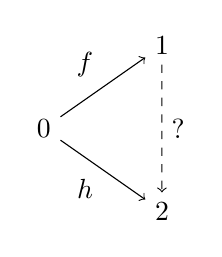
\begin{tikzpicture}[scale=1.5]
\node (0) at (0,0) {$0$};
\node (1) at (1,0.7) {$1$};
\node (2) at (1,-0.7) {$2$};
\draw[->] (0) -- node[above left] {$f$} (1);
\draw[->] (0) -- node[below left] {$h$} (2);
\draw[->, dashed] (1) -- node[right] {$?$} (2);
\end{tikzpicture}
\end{center}

The horn $\Lambda_0^2$ specifies:
\begin{itemize}
\item An edge $f : 0 \to 1$.
\item An edge $h : 0 \to 2$.
\item The vertex $0$ is the common source.
\end{itemize}

A \textbf{filler} provides an edge $g : 1 \to 2$ such that the 2-simplex witnesses $h \simeq g \circ f$. But notice: this is not ``composing $f$ and $g$''---we don't \emph{have} $g$ yet. We have $f$ and the ``answer'' $h$, and we're asking: can we \emph{factor} $h$ through $f$? This is division: $g = h / f$, or equivalently, ``$f$ can be cancelled from $h$.''

In a Kan complex, such factorizations always exist---which implies every morphism is invertible (you can always ``divide''). In a quasi-category, outer horn fillers are \emph{not} guaranteed; they exist precisely when $f$ happens to be an equivalence.

\subsubsection{Higher Inner Horns: Associativity and Coherence}

For $n = 3$ (a tetrahedron with vertices $0, 1, 2, 3$), the inner horns are $\Lambda_1^3$ and $\Lambda_2^3$.

Consider $\Lambda_1^3$. The missing face is the one opposite vertex $1$: the triangle $\{0, 2, 3\}$. The horn includes:
\begin{itemize}
\item Edges $0 \to 1$, $1 \to 2$, $1 \to 3$, $2 \to 3$, $0 \to 2$, $0 \to 3$.
\item Faces $\{0,1,2\}$, $\{0,1,3\}$, $\{1,2,3\}$.
\end{itemize}

Filling this horn produces the face $\{0,2,3\}$ and a 3-simplex witnessing coherence among the various 2-simplices. This encodes \emph{associativity}: given that $(f \circ g) \circ h$ and $f \circ (g \circ h)$ both exist, the filler witnesses they cohere.

In general: inner horns at dimension $n$ encode $(n-1)$-fold compositional coherence. Dimension 2 is composition; dimension 3 is associativity; dimension 4 is the ``pentagon'' coherence for associativity of associativity; and so on.

\subsubsection{Summary: The Inner/Outer Distinction}

\begin{center}
\begin{tabular}{lll}
\textbf{Horn type} & \textbf{What it asks} & \textbf{Categorical meaning} \\
\hline
Inner ($0 < i < n$) & Can we compose? & Composition exists \\
Outer ($i = 0$ or $n$) & Can we divide/factor? & Characterizes equivalences \\
\end{tabular}
\end{center}

\begin{definition}[Inner horn class]
\label{def:inner-horn-class}
For a simplicial object $K$, define the class of \textbf{inner horns} by
\[
\mathrm{Horn}_{\mathrm{inner}}(K) := \coprod_{n \ge 2} \coprod_{0<i<n} \mathrm{Hom}(\Lambda_i^n, K).
\]
Note: there are no inner horns at dimension $n = 1$ (since $0 < i < 1$ is empty).
\end{definition}

\begin{definition}[Kan complex]
A simplicial set $K$ is a \textbf{Kan complex} if every horn $\Lambda_i^n \to K$ (inner or outer) admits a filler $\Delta^n \to K$.
\end{definition}

\begin{definition}[Quasi-category]
A simplicial set $Q$ is a \textbf{quasi-category} (or $\infty$-category) if every \emph{inner} horn $\Lambda_i^n \to Q$ with $0 < i < n$ admits a filler.
\end{definition}

\begin{remark}[The categorical landscape]
Kan complexes model $\infty$-groupoids: all morphisms are invertible up to coherent homotopy. Quasi-categories model $(\infty,1)$-categories: composition exists and is coherent, but morphisms need not be invertible. The distinction matters: meaning-space has directionality. Understanding does not always reverse; semantic paths are not always invertible.
\end{remark}

\subsection{Where OHTT Sits}

OHTT assumes meaning-space is generally \emph{not Kan}. This much is obvious: semantic relations are directional, non-invertible, path-dependent. But the quasi-categorical condition is also too strong. Consider:

\begin{example}[Failure of inner horn filling]
The horn $\Lambda_1^2$ for the composable pair
\[
\textit{Justice} \xrightarrow{} \textit{Equality} \xrightarrow{} \textit{Sameness}
\]
does not fill: there is no coherent composite edge from \textit{Justice} to \textit{Sameness}. This is an inner horn ($i=1$, $n=2$) that fails to fill. Meaning-space is not quasi-categorical.
\end{example}

\begin{example}[Higher inner horn failure]
Even when 2-dimensional composition succeeds locally, associativity (the $\Lambda_i^3$ inner horns for $0 < i < 3$) may fail. The hermeneutic circle---Author's intention, Historical context, Reader's horizon, Textual meaning---exhibits path-dependent composition where the order of interpretation matters. The 3-horn does not fill; associativity is gapped.
\end{example}

The point of OHTT is to treat such failures as \emph{positive witnessed structure} rather than error. We do not demand that meaning-space be quasi-categorical; we develop a logic that can speak precisely about where inner horns fill and where they do not.

\subsection{The Three-Layer Semantics}

This observation leads to a crucial architectural distinction that will inform the entire book:

\begin{description}
\item[Layer 0: Raw simplicial object.] The type structure $T(X)$ built from corpus $C$ by construction method $X$. This is combinatorial data: vertices, edges, higher simplices determined by the construction.

\item[Layer 1: Witness-marking.] The Semantic Witness Log (developed below and in Chapter 3) marks some horns as coherent ($\coh$), some as gapped ($\gap$), most as uninscribed. This is the actual semantics of OHTT: witnessed, indexed, partial.

\item[Layer 2: Quasi-categorical completion.] For any simplicial set $K$, there exists a quasi-category $K^{\mathrm{qc}}$ and a map $\eta_K : K \to K^{\mathrm{qc}}$ that is a categorical equivalence (in the Joyal model structure). This completion freely adjoins fillers for all inner horns, providing an \emph{analytic envelope} in which composition is everywhere available.
\end{description}

\begin{theorem}[Existence of quasi-categorical completion]
\label{thm:qc-completion}
Every simplicial set $K$ admits a quasi-categorical completion $\eta_K : K \to K^{\mathrm{qc}}$ where $K^{\mathrm{qc}}$ is a quasi-category and $\eta_K$ is a categorical equivalence.
\end{theorem}

\begin{proof}[Proof sketch]
This is fibrant replacement in the Joyal model structure on simplicial sets. See \cite{joyal2008notes} for the original construction and \cite{lurie2009higher} for the development in the context of $(\infty,1)$-categories.
\end{proof}

\begin{remark}
The completion $K^{\mathrm{qc}}$ is not canonical on the nose (it depends on choices of fibrant
replacement), but it is canonical up to categorical equivalence.
\end{remark}

\begin{remark}[The crucial policy]
The completion does not overwrite the witness-marking. It provides a second, distinct notion of ``filler exists'':
\begin{itemize}
\item In $T(X)$: a filler exists if the type structure contains it (decidable for algorithmic constructions).
\item In $T(X)^{\mathrm{qc}}$: a filler exists by closure---the completion has freely adjoined it.
\item In the SWL: a filler is \emph{witnessed coherent} if a record $p : \coh(H)$ exists under some configuration $V$.
\end{itemize}
These three notions are distinct. The logical win of OHTT is precisely this separation: we can reason about what \emph{would} compose (in the envelope) while tracking what \emph{has been witnessed} to cohere (in the log).
\end{remark}

\subsection{Compositional Inner Horns}

Two lemmas make the compositional interpretation precise:

\begin{lemma}[The compositional inner horn]
\label{lem:comp-horn}
A map $H : \Lambda_1^2 \to K$ is equivalently the data of a composable pair of edges $x \xrightarrow{f} y \xrightarrow{g} z$ in $K$, together with the common vertex $y$. A filler $\sigma : \Delta^2 \to K$ extending $H$ exhibits a candidate composite edge $h : x \to z$ together with the 2-simplex witnessing $h \simeq g \circ f$.
\end{lemma}

\begin{lemma}[Existence of composites in a quasi-category]
\label{lem:qc-composites}
If $Q$ is a quasi-category, then every inner 2-horn $H : \Lambda_1^2 \to Q$ admits a filler. Hence every composable pair of 1-simplices in $Q$ admits a composite, well-defined up to coherent higher data.
\end{lemma}

These lemmas clarify what OHTT is doing: tracking, horn by horn, which compositions succeed and which fail, without assuming the quasi-categorical condition that would guarantee all compositions succeed.

\subsection{Why This Matters for the Book}

The quasi-categorical framing provides several things the book needs:

\begin{enumerate}
\item \textbf{Compositional semantics.} The inner/outer distinction makes precise what kind of coherence failure we're tracking. When we say ``the horn is gapped,'' we can now specify: is it an inner horn (composition failed) or an outer horn (invertibility failed)? For meaning-space, the interesting failures are primarily inner.

\item \textbf{A canonical closure.} The completion $T(X)^{\mathrm{qc}}$ provides a well-defined envelope for reasoning about implied structure. This is analogous to deductive closure in logic: we can ask ``what would follow if we closed under composition?'' without claiming those consequences were ever witnessed.

\item \textbf{Preparation for Chapter 6.} The homotopy colimit construction that defines the Self requires a homotopy-coherent gluing of viewpoints. After quasi-categorical completion, the hocolim presents the $\infty$-categorical colimit---the universal way to hold multiple partial, conflicting viewpoints together. This is the categorical justification for why the Self construction works.
\end{enumerate}

The slogan ``meaning-space is not Kan'' now admits refinement:
\begin{itemize}
\item Not Kan: no reason to expect invertibility of semantic paths.
\item Often not quasi-categorical: composition itself can rupture.
\item But quasi-categorical completion exists as envelope: a disciplined way to reason about implied compositional structure.
\end{itemize}

OHTT is the logic of the gap between Layer 1 (witnessed marking) and Layer 2 (completed envelope). The gap is not error; it is the space where meaning lives.


%% ============================================================
%% THE HORN HIERARCHY
%% ============================================================

\section{The Horn Hierarchy: Bewilderment at Every Level}

Bewilderment is not a single phenomenon but a \emph{hierarchy}. The non-Kan character of semantic space means that gaps can appear at any level. This is not a technicality but the heart of the matter: \emph{bewilderment lives in the higher faces}.

\subsection{Dimension 1: Path Coherence}

At $n = 1$, the question is simple: given objects $x$ and $y$, does a path connect them? Do they cohere?

For the sonnets with basin structure: $x$ and $y$ cohere if they fall in the same basin; they are gapped if they fall in different basins.

This is the simplest case, and much of our empirical work restricts to $n = 1$. But path-level coherence is only the beginning.

\subsection{Dimension 2: Composition}

At $n = 2$, we have the transport horn. Given two witnessed coherences $p : x \to y$ and $q : y \to z$, we ask: does $x$ cohere with $z$? Does composition succeed?

In a Kan complex, the answer is always yes. But meaning-space is not Kan.

\textbf{Example (Justice-Equality-Sameness):}
\begin{itemize}
\item $p$: \textit{Justice} coheres with \textit{Equality}
\item $q$: \textit{Equality} coheres with \textit{Sameness}
\item Missing: Does \textit{Justice} cohere with \textit{Sameness}?
\end{itemize}

The answer is gapped. Justice is not sameness; treating everyone identically is not treating everyone justly. The 2-horn witnesses this gap: local coherences that do not compose into global coherence.

At $n = 2$, bewilderment is compositional: I can get from $x$ to $y$ and from $y$ to $z$, but the composition does not cohere.

\subsection{Dimension 3: Associativity}

At $n = 3$, we encounter the associativity horn. Suppose we have $p : w \to x$, $q : x \to y$, $r : y \to z$, and compositions succeed pairwise. Does it matter which way we associate? Can we coherently relate $w$ to $z$?

\textbf{Example (Hermeneutic Circle):}
Consider four interpretive positions: Author's intention ($w$), Historical context ($x$), Reader's horizon ($y$), Textual meaning ($z$). Suppose local coherences exist and pairwise compositions succeed. But the two routes from Author's intention to Textual meaning may yield different coherences. The associativity horn is gapped. The hermeneutic circle does not close; the path you take \emph{matters}.

At $n = 3$, bewilderment becomes path-dependent. Local coherences exist, triangles fill, but when I try to hold the entire four-term structure together, the order of composition matters.

\subsection{Higher Dimensions}

The pattern continues. At each dimension $n$, we ask whether $(n-1)$-level coherences compose into $n$-level coherence.

The key insight: I may have path coherence ($n = 1$), compositional coherence ($n = 2$), and still be gapped at associative coherence ($n = 3$). The lower coherences exist; the higher coherence that would bind them does not. This is bewilderment in the higher faces: the local makes sense, the global eludes.

In subsequent chapters, we work primarily at $n = 1$ and $n = 2$ for empirical tractability. But the logic supports witnessing at all levels.


%% ============================================================
%% WITNESSING DISCIPLINES
%% ============================================================

\section{Witnessing Disciplines}
\label{sec:ohtt-witnessing}

The type structure specifies the space. The \textbf{witnessing configuration} specifies how verdicts are produced at horns in that space. This is the second axis of the apparatus, orthogonal to the first.

One could treat the witness as an external oracle: a black box that emits verdicts, indexed by an opaque label. The calculus would still function---judgments would be indexed by labels, surplus would arise when labels disagree. But this minimalism misses what we are attempting. The witness is not exogenous to meaning-constitution; the witness is part of the constructive assemblage. The proof term $p : \coh(H)$ does not merely record that coherence was witnessed; it records \emph{how} coherence was witnessed, by \emph{what kind of entity}, under \emph{what methodology}, with \emph{what parameters}. This is the constructivist commitment taken seriously: the proof is not mere certificate but the actual construction, and the construction includes the constructor.

We therefore structure the witnessing configuration to carry as much data as the investigation requires. The schema we adopt here is one choice among many possible; the calculus is parameterized by such choices, not wedded to a fixed structure.

\begin{definition}[Witnessing Configuration]
A \textbf{witnessing configuration} is a record $V := (D, w, \kappa)$, where:
\begin{itemize}
\item $D$ is a \textbf{discipline taxonomy}---a path through a declared classification of witnessing methods,
\item $w$ is a \textbf{witness taxonomy}---a path through a declared classification of witness instances,
\item $\kappa$ packages \textbf{parameters} for the particular application.
\end{itemize}
\end{definition}

The discipline taxonomy $D$ classifies \emph{what kind} of witnessing occurs. At the coarsest level, we distinguish three branches:

\textbf{Algorithmic} ($D = \mathsf{Raw}.\_$): The verdict is computed from the apparatus by a specified procedure. The taxonomy branches further: $\mathsf{Raw}.\mathsf{VietorisRips}$ for threshold-based simplicial construction, $\mathsf{Raw}.\mathsf{kNN}$ for $k$-nearest-neighbor graphs, $\mathsf{Raw}.\mathsf{PH}$ for persistent homology pipelines, and so on. Available only for decidable type structures.

\textbf{Human} ($D = \mathsf{Human}.\_$): The verdict is produced by human judgment. The taxonomy branches: $\mathsf{Human}.\mathsf{Expert}$ for domain specialists, $\mathsf{Human}.\mathsf{Annotator}$ for trained labelers, $\mathsf{Human}.\mathsf{Naive}$ for uninstructed readers. Further branches are possible---by training protocol, by cultural background, by institutional affiliation.

\textbf{Model-based} ($D = \mathsf{LLM}.\_$): The verdict is produced by a language model under a prompt protocol. The taxonomy branches by architecture family ($\mathsf{LLM}.\mathsf{GPT}$, $\mathsf{LLM}.\mathsf{Claude}$, $\mathsf{LLM}.\mathsf{Llama}$), by scale, by fine-tuning lineage.

The witness taxonomy $w$ classifies \emph{which} witness of a given kind. For algorithmic disciplines, $w$ names the specific implementation or version. For human disciplines, $w$ names the individual (or anonymized identifier). For model-based disciplines, $w$ names the checkpoint, quantization level, and deployment context. The taxonomy may be as shallow as a single label or as deep as the investigation requires.

The parameters $\kappa$ specify \emph{how} the witness was applied in this instance: similarity threshold $\epsilon$, prompt template, temperature, context window, rubric, time budget. These are the arguments to the witnessing act.

\begin{remark}[Why structure $V$?]
One could collapse $(D, w, \kappa)$ into a single label and lose no expressive power at the level of individual judgments. The value of the structure emerges when we compare judgments across witnesses. Surplus is not merely ``they disagree'' but ``they disagree along this axis'': two $\mathsf{Raw}$ witnesses with different $\epsilon$ disagree about threshold; a $\mathsf{Human}.\mathsf{Expert}$ and an $\mathsf{LLM}.\mathsf{Claude}$ disagree about something deeper. The taxonomic structure of $D$ and $w$ makes these distinctions speakable. When we later glue witness logs via homotopy colimit, the structure of $V$ organizes the gluing---recognizing which disagreements are along the same axis and which are orthogonal.
\end{remark}

The crucial principle: \textbf{type structure and witnessing configuration are orthogonal}. The same horn may be witnessed under different configurations. Different configurations may yield different verdicts for the same horn. This divergence is not error---it is \textbf{surplus}, the formal trace of meaning exceeding any single type-configuration pair.


%% ============================================================
%% JUDGMENT FORMS
%% ============================================================

\section{Judgment Forms and Witness Records}
\label{sec:ohtt-judgments}

With type structures, horns, and disciplines in view, we can now present the judgment forms.

\begin{definition}[Polarized OHTT Judgments]
Given type structure $T(X)$, witnessing configuration $V$, and transport situation $H$, OHTT admits two polarized judgment forms:
\[
\coh_{T(X)}^{V}(H)
\qquad\text{and}\qquad
\gap_{T(X)}^{V}(H).
\]
Read: ``under $(T(X),V)$ the situation $H$ is witnessed coherent'' and ``under $(T(X),V)$ the situation $H$ is witnessed gapped.''
\end{definition}

\textbf{Coherence}: A witness exhibits a filler---a path, a composition, a higher simplex that completes the partial structure. Under this type structure and discipline, the horn is realized.

\textbf{Gap}: A witness marks $H$ as a site of witnessed openness. Under this type structure and discipline, no admissible filler is present. The gap witness does not assert impossibility in any absolute sense; it marks present openness without foreclosing future filling.

\begin{definition}[Uninscribed]
When neither coherence nor gap has been witnessed for $H$ under $(T(X), V)$, the horn is \textbf{uninscribed}---no entry exists in the witness record. This is not a third judgment; it is absence of judgment.
\end{definition}

The distinction between gapped and uninscribed is crucial. An uninscribed horn is untouched---we haven't stood at that altar. A gapped horn is one we have entered and found open. The witnessing is the shahādah of rupture.

\begin{definition}[Witness Record]
A \textbf{witness record} $p$ inhabiting a judgment packages:
\begin{itemize}
\item situation specification (dimension, index, participating objects),
\item type-structure identifier (construction method $X$ and parameters),
\item witnessing configuration $V$,
\item verdict polarity ($\coh$ or $\gap$),
\item evidence (filler, computation trace, or rationale),
\item metadata sufficient for re-audit.
\end{itemize}
We write $p : \coh_{T(X)}^{V}(H)$ or $p : \gap_{T(X)}^{V}(H)$.
\end{definition}

\begin{definition}[Path-level notation]
For $n=1$, we write:
\[
\coh_{T(X)}^{V}\; p : x =_{T(X)} y
\qquad\text{or}\qquad
\gap_{T(X)}^{V}\; p : x =_{T(X)} y
\]
as shorthand for a witnessed verdict about whether the edge from $x$ to $y$ is admissible.
\end{definition}

\subsection{The Subject Inside the Proof Term}

The received view dreams of inference without inferrer, proof without prover. We refuse this dream.

The witness record $p$ contains not just the verdict but who witnessed, under what conditions, with what stance. Even for fully algorithmic Raw witnessing, the subject is present: someone chose this type structure, someone authorized this apparatus, someone accepts this verdict as their inscription. The machine computes; the subject witnesses.

For Human or LLM disciplines, the subject's presence becomes richer. The witness record includes the subject's trajectory, their attunement to this domain, their rationale for entering this horn. The contemplation is part of the data.

This is what Chapter 1 meant by ``the subject inside the proof term.'' The witness $p$ is not a generic certificate. It is \emph{this} witness, from \emph{this} subject, with \emph{this} stance.


%% ============================================================
%% WITNESS-MARKED SIMPLICIAL OBJECTS
%% ============================================================

\section{Witness-Marked Simplicial Objects}
\label{sec:marked-objects}

The judgment forms of the preceding section---$\coh_{T(X)}^V(H)$ and $\gap_{T(X)}^V(H)$---can be repackaged into a single mathematical object: a simplicial set equipped with a \emph{polarized marking} of its horns. This repackaging is not merely notational; it provides the categorical semantics that makes OHTT's constructivist commitments precise and prepares for the dynamic extension in Chapter 3.

\subsection{Polarized Horn Markings}

\begin{definition}[Horn class]
For a simplicial object $K$, let $\mathrm{Horn}(K)$ denote the class of all transport situations:
\[
\mathrm{Horn}(K) := \coprod_{n \geq 1} \coprod_{0 \leq i \leq n} \mathrm{Hom}(\Lambda_i^n, K).
\]
\end{definition}

\begin{definition}[Polarized horn marking]
\label{def:polarized-marking}
A \textbf{polarized marking} on a simplicial object $K$ is a pair of subsets
\[
M^+(K),\; M^-(K) \;\subseteq\; \mathrm{Horn}(K)
\]
such that $M^+(K) \cap M^-(K) = \emptyset$. Elements of $M^+(K)$ are \emph{coherence-marked horns}; elements of $M^-(K)$ are \emph{gap-marked horns}. Horns in neither set are \emph{uninscribed}.
\end{definition}

\begin{definition}[Witness-marked simplicial object]
A \textbf{witness-marked simplicial object} is a pair $(K, M^\pm)$ where $K$ is a simplicial set and $M^\pm = (M^+, M^-)$ is a polarized marking on $K$.
\end{definition}

This definition makes precise what a type structure ``looks like'' after witnessing has occurred. The SWL is not a separate bookkeeping device; it \emph{is} the marking. The polarized marking is the geometric residue of all the shahādahs spoken at all the altars.

\subsection{From SWL to Marking}

\begin{definition}[Induced marking from SWL]
\label{def:induced-marking}
Given a type structure $T(X)$ and witnessing configuration $V$, the Semantic Witness Log induces a polarized marking $M^\pm_{X,V}(T(X))$ by:
\begin{align*}
H \in M^+_{X,V}(T(X)) &\quad\Longleftrightarrow\quad \exists\, p : \coh_{T(X)}^V(H) \text{ in the log} \\
H \in M^-_{X,V}(T(X)) &\quad\Longleftrightarrow\quad \exists\, p : \gap_{T(X)}^V(H) \text{ in the log}
\end{align*}
The Exclusion principle guarantees these sets are disjoint.
\end{definition}

\begin{remark}[Proof relevance preserved]
The marking records \emph{that} a horn is coherent or gapped, not the specific witness record. Proof relevance is preserved in the full SWL; the marking is a projection that forgets the evidence while retaining the verdict. For some purposes (e.g., computing coherence rates) the marking suffices; for others (e.g., auditing, understanding \emph{why} a verdict was reached) the full witness record is needed.
\end{remark}

\subsection{Partial Fibrancy}

The marking allows us to speak precisely about \emph{how fibrant} a type structure is under a given witnessing regime.

\begin{definition}[Inner-coherence rate (empirical)]
Fix a finite inspected set $S \subseteq \mathrm{Horn}_{\mathrm{inner}}(K)$ of inner horns.
The \textbf{inner-coherence rate} on $S$ is
\[
\rho^+(K,M^\pm;S) := \frac{|M^+(K)\cap S|}{|(M^+(K)\cup M^-(K))\cap S|}.
\]
This measures what fraction of inspected inner horns are coherent among those that have been witnessed at all.
\end{definition}

\begin{definition}[Partially inner-fibrant]
A witness-marked object $(K, M^\pm)$ is \textbf{partially inner-fibrant} if there exists at least one
inner horn witnessed coherent:
\[
M^+(K)\cap \mathrm{Horn}_{\mathrm{inner}}(K)\neq \emptyset.
\]
It is \textbf{fully inner-fibrant relative to the marking} if every inscribed inner horn is coherent-marked:
\[
M^-(K)\cap \mathrm{Horn}_{\mathrm{inner}}(K)=\emptyset.
\]
\end{definition}

\begin{remark}[OHTT as the logic of partial inner-fibrancy]
OHTT is precisely the logic of partially inner-fibrant objects. We do not assume full fibrancy (which would make every horn fillable) or even full inner-fibrancy (which would make every inner horn fillable). We track, horn by horn, what has been witnessed and what remains open.
\end{remark}

\subsection{The Category of Marked Objects}

Witness-marked simplicial objects form a category, which will matter when we glue viewpoints in Chapter 6.

\begin{definition}[Morphism of marked objects]
A \textbf{morphism} $(K, M^\pm_K) \to (L, M^\pm_L)$ is a simplicial map $f : K \to L$ such that:
\begin{itemize}
\item $f$ carries coherent-marked horns to coherent-marked horns: if $H \in M^+_K$, then $f \circ H \in M^+_L$.
\item $f$ carries gap-marked horns to gap-marked horns: if $H \in M^-_K$, then $f \circ H \in M^-_L$.
\end{itemize}
\end{definition}

\begin{remark}[Morphisms preserve witnessed structure]
A morphism of marked objects is a simplicial map that respects the witnessing. It does not matter whether the target has additional marked horns; what matters is that the image of a witnessed horn retains its polarity. This is the categorical expression of the constructivist commitment: witnessed structure is preserved under maps.
\end{remark}

\subsection{Time-Indexed Markings (Preview)}

Chapter 3 extends this apparatus to handle evolving texts. The key move: index the marking by \emph{two} times.

\begin{definition}[Time-indexed marking (preview)]
Given an evolving type structure $\{T(X)_\tau\}_{\tau \in \mathcal{T}}$ and witnessing configuration $V$, the SWL determines a family of markings:
\[
M^\pm_{X,V,\tau_{\mathrm{tgt}},\tau_{\mathrm{wit}}}(T(X)_{\tau_{\mathrm{tgt}}})
\]
indexed by target time $\tau_{\mathrm{tgt}}$ (when the type structure is evaluated) and witness time $\tau_{\mathrm{wit}}$ (when the witnessing occurred).
\end{definition}

This is the precise formal definition of what the book calls a ``time-indexed, witness-indexed partially fibrant object'': it is the family $\{M^\pm_{X,V,\tau_{\mathrm{tgt}},\tau_{\mathrm{wit}}}\}$ of polarized markings, varying over both temporal indices.


%% ============================================================
%% CORRESPONDENCES AND SURPLUS
%% ============================================================

\section{Correspondences and Surplus}

When we build multiple type structures from the same corpus---one using embeddings, one using persistent homology, or the same method with different parameters---we need a way to compare horns across constructions.

\begin{definition}[Horn Correspondence]
Let $T(X)$ and $T(Y)$ be type structures from the same corpus. A \textbf{horn correspondence scheme} is a declared rule which, given a horn $H:\Lambda_i^n \to T(X)$, produces (when possible) a horn $H':\Lambda_i^n \to T(Y)$ referring to the ``same underlying vertices'' under an identification rule.
\end{definition}

Correspondences are not canonical. Different schemes encode different interpretive choices. OHTT treats correspondence as declared structure, not background magic.

\begin{definition}[Surplus]
Given two type-discipline pairs $(T(X),V)$ and $(T(Y),W)$ and corresponding situations $(H,H')$, the possibility of differing verdicts
\[
\coh_{T(X)}^{V}(H) \quad\text{and}\quad \gap_{T(Y)}^{W}(H')
\]
is called \textbf{surplus}. Surplus is recorded, not suppressed: it is the formal trace of meaning exceeding any single construction or discipline.
\end{definition}

Surplus is not noise to be eliminated. It is data to be tracked. The witness log records all judgments; the divergences remain visible; the excess of meaning over measurement is preserved as structure.

The question of how to \emph{glue} divergent verdicts---how to construct a coherent picture from witnesses that disagree---is deferred to Chapter 6, where the homotopy colimit provides the apparatus for holding together what does not fully cohere.


%% ============================================================
%% SURPLUS AS CATEGORICAL STRUCTURE
%% ============================================================

\section{Surplus as Categorical Structure}
\label{sec:surplus-categorical}

The preceding section introduced surplus informally: two witnessing regimes disagree on corresponding horns. This section makes surplus categorically precise and explains why homotopy colimits (Chapter 6) are the right tool for handling it.

\subsection{Surplus as Marking Divergence}

\begin{definition}[Surplus witness]
\label{def:surplus-witness}
Let $(T(X), V_1)$ and $(T(Y), V_2)$ be two type-configuration pairs with a horn correspondence $H \leftrightarrow H'$. A \textbf{surplus witness} is a pair $(p, q)$ where:
\begin{itemize}
\item $p : \coh_{T(X)}^{V_1}(H)$ and $q : \gap_{T(Y)}^{V_2}(H')$, or
\item $p : \gap_{T(X)}^{V_1}(H)$ and $q : \coh_{T(Y)}^{V_2}(H')$.
\end{itemize}
The corresponding horns receive opposite verdicts under the two regimes.
\end{definition}

In the language of marked objects: surplus is where two markings disagree on corresponding horns. If we have marked objects $(T(X), M^\pm_1)$ and $(T(Y), M^\pm_2)$ with a correspondence that identifies horn $H$ with horn $H'$, then surplus at this site means:
\[
H \in M^+_1 \;\land\; H' \in M^-_2 \qquad\text{or}\qquad H \in M^-_1 \;\land\; H' \in M^+_2.
\]

\subsection{Why Surplus Cannot Be Resolved}

The temptation is to resolve surplus: choose one verdict, suppress the other, produce a consistent picture. OHTT refuses this temptation. The refusal has both philosophical and mathematical grounds.

\textbf{Philosophical ground.} The Type-Discipline Orthogonality principle asserts that construction method and witnessing configuration are independent axes. No type-configuration pair is privileged. To resolve surplus by choosing one verdict is to privilege one regime over another---a move the logic does not license.

\textbf{Mathematical ground.} Different markings encode different aspects of semantic structure. $T(\mathsf{embed})$ sees local similarity; $T(\mathsf{bar})$ sees global topology. A horn coherent under one may be gapped under the other not because one is ``wrong'' but because they are measuring different things. Forcing agreement would destroy information.

\subsection{Gluing Without Erasing: The Homotopy Colimit}

The right way to combine divergent marked objects is not to force agreement but to \emph{glue along correspondences while preserving disagreement}. This is precisely what the homotopy colimit does.

\begin{definition}[Diagram of marked objects]
A \textbf{diagram of marked objects} over an indexing category $I$ is a functor
\[
D : I \longrightarrow \mathsf{sSet}^{\pm}
\]
where $\mathsf{sSet}^{\pm}$ is the category of witness-marked simplicial objects.
\end{definition}

\begin{definition}[Homotopy colimit of marked objects]
The \textbf{homotopy colimit} $\mathrm{hocolim}_I\, D$ is a marked simplicial object that:
\begin{itemize}
\item contains a copy of each $D(i)$,
\item glues these copies along the morphisms of $I$ (the correspondences),
\item preserves the marking structure: a horn in $\mathrm{hocolim}_I\, D$ is coherent-marked if it came from a coherent-marked horn in some $D(i)$, and similarly for gap-marked.
\end{itemize}
\end{definition}

\begin{remark}
Formally: let $U:\mathsf{sSet}^{\pm}\to\mathsf{sSet}$ forget the marking.
Define $\operatorname{hocolim}_I D$ as $\operatorname{hocolim}_I (U\circ D)$ in $\mathsf{sSet}$,
equipped with the \emph{smallest} marking for which each structure map $D(i)\to\operatorname{hocolim}_I D$
preserves polarity. New simplices created by the hocolim construction (corridors, higher glue) are
initially uninscribed unless later witnessed.
\end{remark}

The key property: \emph{the hocolim does not force agreement}. If corresponding horns $H$ and $H'$ receive opposite verdicts in $D(i)$ and $D(j)$, then in the hocolim both verdicts are present. The correspondence is recorded as a ``seam''---a site where regimes disagree. The seam is structure, not error.

\begin{remark}[Seams as positive data]
In ordinary colimits, identified points become equal---the colimit ``quotients out'' the correspondence. In homotopy colimits, identified points are connected by paths---the correspondence becomes geometric structure. Seams in the Self (Chapter 6) are precisely these paths: they record where viewpoints touch without forcing them to agree.
\end{remark}

\subsection{Functoriality Failure as Surplus}

There is another way to see surplus: as failure of functoriality.

If we had a single ``true'' marking that all constructions and disciplines approximated, then the correspondence maps would preserve marking: coherent in one regime would imply coherent in the other. Surplus would be impossible.

Surplus is possible precisely because there is no such true marking. Different regimes see different structure. The correspondence maps do not preserve marking; they only preserve \emph{which horn we're talking about}. The marking divergence is the surplus.

\begin{proposition}[Surplus detects functoriality failure]
\label{prop:surplus-functoriality}
Let $\phi : (T(X), V_1) \to (T(Y), V_2)$ be a horn correspondence (identifying corresponding horns across type structures). Surplus at a horn $H$ under $\phi$ is equivalent to:
\[
\phi \text{ does not preserve marking at } H.
\]
\end{proposition}

This makes surplus categorically inevitable: once we admit multiple constructions and disciplines, functoriality of correspondence maps is not guaranteed. The divergences are the price of plurality. OHTT and the hocolim construction (Chapter 6) turn this price into a feature: surplus is data, not defect.

\subsection{Preparation for Chapter 6}

The machinery developed here---marked objects, morphisms that may fail to preserve marking, homotopy colimits that preserve disagreement as seams---is exactly what Chapter 6 needs to construct the Self.

The Self is not a single marked object but the homotopy colimit over all admissible type-configuration pairs. Each pair contributes a viewpoint; the correspondences connect viewpoints; the seams record where viewpoints diverge. The result is a space that holds together what does not fully cohere---the only kind of space adequate to a Self that overflows any single measurement regime.


%% ============================================================
%% GOVERNING PRINCIPLES
%% ============================================================

\section{Governing Principles}
\label{sec:ohtt-principles}

\begin{principle}[Exclusion]
For fixed $T(X)$, $V$, and $H$:
\[
\coh_{T(X)}^{V}(H) \;\land\; \gap_{T(X)}^{V}(H) \;\Rightarrow\; \bot.
\]
Coherence and gap are mutually exclusive for the same horn under the same type-discipline pair.
\end{principle}

\begin{principle}[Proof Relevance]
If $p : \coh_{T(X)}^{V}(H)$ and $p' : \coh_{T(X)}^{V}(H)$, we do not assume $p = p'$. Witness records are proof-relevant: different evidence, stance, or procedure yields different witnesses.
\end{principle}

\begin{principle}[Type-Discipline Orthogonality]
Construction method and witnessing configuration are orthogonal axes. The same horn can be witnessed under multiple configurations; divergence across axes contributes to surplus.
\end{principle}

\begin{principle}[No View from Nowhere]
All claims of coherence or gap are indexed by a declared $(T(X),V)$. Even $\mathsf{Raw}$ is a discipline---a specified procedure with specified parameters.
\end{principle}

\begin{principle}[Constitutive Witnessing]
When the space is not decidable, or when one adopts $\mathsf{Human}$ or $\mathsf{LLM}$, the ``known'' structure is the accumulated set of witness records. Structure is not merely described by witnessing; it is constituted by inscription.
\end{principle}


%% ============================================================
%% VIETORIS-RIPS AND THE FILTRATION FUNCTOR
%% This section commits to VR, develops the ambient-complex
%% reformulation, proves TDA is the decidable fragment of OHTT,
%% and fixes epsilon for the remainder of the book.
%% ============================================================

%% REPLACES the earlier RR_Chapter2_epsilon_insert.tex
%% INSERT IN CHAPTER 2 after "Governing Principles" and before "Summary: What OHTT Achieves"
%% This section commits to VR, develops the epsilon phenomenology,
%% and then makes the key move: the VR filtration IS a functor into sSet^±,
%% unifying TDA with OHTT and formally separating decidable from hermeneutic witnessing.

\section{Vietoris--Rips and the Filtration Functor}
\label{sec:vr-filtration}

The preceding sections developed OHTT at a level of generality that admits
many choices of simplicial structure on embedding space:
Vietoris--Rips complexes, \v{C}ech complexes, alpha complexes,
$k$-nearest-neighbor clique complexes.
We now commit to a default and show that the commitment yields a formal result:
the Vietoris--Rips filtration is a functor into $\mathbf{sSet}^{\pm}$,
and this functor unifies TDA's ``vary the complex'' with OHTT's ``vary the marking''
into a single picture.

\subsection{Vietoris--Rips as Canonical Construction}

The \textbf{Vietoris--Rips complex} $\mathrm{VR}(P, \epsilon)$ on a finite point cloud $P$
in a metric space $(X, d)$ is defined by:
\[
\sigma = \{p_0, \ldots, p_k\} \in \mathrm{VR}(P, \epsilon)
\quad\Longleftrightarrow\quad
\forall\, i, j:\; d(p_i, p_j) \leq \epsilon.
\]
We adopt VR as the canonical construction for $T(\mathsf{embed})$ for three reasons.

First, \emph{universality in TDA}: Vietoris--Rips is the standard construction
in topological data analysis~\cite{carlsson2009topology, edelsbrunner2010computational},
with well-studied phase-transition behavior
on random point clouds~\cite{kahle2011random, bobrowski2018topology}.
Using VR allows the book's results to be directly compared with the TDA literature.

Second, \emph{computability}: VR depends only on pairwise distances.
For embedding spaces with cosine similarity,
$d_{\cos}(p_i, p_j) \leq \epsilon$ is equivalent to
$\mathrm{sim}(p_i, p_j) \geq 1 - \epsilon$.
Efficient algorithms exist~\cite{edelsbrunner2010computational}
and are implemented in standard libraries (Ripser, GUDHI).

Third, \emph{philosophical transparency}: the single parameter $\epsilon$
has a clear semantic interpretation as the threshold of witnessed proximity.
The all-pairs condition ($\sigma$ exists iff \emph{every} pair passes the test)
is precisely the compositional requirement
that connects simplicial construction to the horn-filling semantics of OHTT.


\subsection{The Ambient Complex and Its Markings}
\label{subsec:ambient}

The standard TDA perspective on the VR filtration is:
as $\epsilon$ increases, the simplicial complex grows.
New edges appear, new triangles form, new higher simplices are born.
The object of study is the \emph{nested family of complexes}
$\{\mathrm{VR}(P, \epsilon)\}_{\epsilon \geq 0}$.

OHTT suggests a different perspective.
Fix the \textbf{full simplex} $\Delta^N$ on the $N$ vertices of the corpus---the maximal
type structure in which every possible simplex exists.
Now let $\epsilon$ determine not which simplices exist,
but which horns are \emph{marked}:

\begin{definition}[VR-induced marking at scale $\epsilon$]
\label{def:vr-marking}
Let $P = \{p_1, \ldots, p_N\}$ be a corpus of embedding vectors and $\epsilon \geq 0$.
Define the polarized marking $M^{\pm}_\epsilon$ on $\Delta^N$ by:
\begin{itemize}
\item A horn $H : \Lambda^n_i \to \Delta^N$ is \textbf{coherence-marked} at $\epsilon$
if every face of $H$ and the filler face all belong to $\mathrm{VR}(P, \epsilon)$:
\[
H \in M^+_\epsilon
\quad\Longleftrightarrow\quad
\text{all faces of } H \text{ are in } \mathrm{VR}(P,\epsilon)
\;\text{and}\;
\text{the filler is in } \mathrm{VR}(P,\epsilon).
\]
\item A horn $H$ is \textbf{gap-marked} at $\epsilon$
if all faces of $H$ belong to $\mathrm{VR}(P, \epsilon)$ but the filler does not:
\[
H \in M^-_\epsilon
\quad\Longleftrightarrow\quad
\text{all faces of } H \text{ are in } \mathrm{VR}(P,\epsilon)
\;\text{and}\;
\text{the filler is not in } \mathrm{VR}(P,\epsilon).
\]
\item A horn $H$ is \textbf{uninscribed} at $\epsilon$
if at least one face of $H$ does not belong to $\mathrm{VR}(P, \epsilon)$.
The horn cannot even be posed at this scale.
\end{itemize}
\end{definition}

\begin{remark}[Recovering VR from the marking]
The VR complex at $\epsilon$ is recovered as the
\emph{coherence subcomplex}: the largest subcomplex of $\Delta^N$
whose inner horns are all coherence-marked.
In the other direction, the marking $M^{\pm}_\epsilon$
is determined by the VR complex at $\epsilon$.
The two perspectives carry the same information.
What changes is the emphasis:
TDA emphasizes which simplices exist;
OHTT emphasizes which horns are witnessed and how.
\end{remark}

\begin{remark}[Gap as positive witness, not absence]
In the standard TDA perspective, a missing simplex is a non-event.
In the OHTT perspective, a gap-marked horn is a \emph{positive datum}:
the horn was posable (all its faces exist at this scale)
and found to be unfillable.
This is the shahādah of rupture---gap is not the absence of coherence
but the witnessing of openness.
The ambient-complex formulation makes this distinction concrete:
gap-marks are not holes in the complex but inscriptions on a fixed object.
\end{remark}


\subsection{The Filtration Functor}
\label{subsec:filtration-functor}

The key formal observation:

\begin{proposition}[VR filtration as a functor into $\mathbf{sSet}^{\pm}$]
\label{prop:vr-functor}
The assignment $\epsilon \mapsto (\Delta^N, M^{\pm}_\epsilon)$ defines a functor
\[
\Phi_P : (\mathbb{R}_{\geq 0}, \leq) \longrightarrow \mathbf{sSet}^{\pm},
\]
where $(\mathbb{R}_{\geq 0}, \leq)$ is viewed as a poset category.
For $\epsilon_1 \leq \epsilon_2$, the morphism
$\Phi_P(\epsilon_1 \leq \epsilon_2)$
is the identity on $\Delta^N$ with the property that:
\begin{enumerate}
\item Every $\coh$-marked horn at $\epsilon_1$ remains $\coh$-marked at $\epsilon_2$.
\item Every $\gap$-marked horn at $\epsilon_1$ is either $\coh$-marked or $\gap$-marked at $\epsilon_2$
(it may be ``healed'' or it may persist, but it cannot become uninscribed).
\item Every uninscribed horn at $\epsilon_1$ may become $\coh$-marked, $\gap$-marked,
or remain uninscribed at $\epsilon_2$.
\end{enumerate}
\end{proposition}

\begin{proof}
We must show that the identity map $\mathrm{id} : \Delta^N \to \Delta^N$
is a morphism in $\mathbf{sSet}^{\pm}$ from $(\Delta^N, M^{\pm}_{\epsilon_1})$
to $(\Delta^N, M^{\pm}_{\epsilon_2})$---that is,
it preserves both $\coh$ and $\gap$ markings.

$\coh$-preservation (1):
If $H \in M^+_{\epsilon_1}$, then all faces and the filler of $H$
belong to $\mathrm{VR}(P, \epsilon_1) \subseteq \mathrm{VR}(P, \epsilon_2)$.
Hence $H \in M^+_{\epsilon_2}$.

$\gap$-preservation (2):
If $H \in M^-_{\epsilon_1}$, then all faces of $H$ are in $\mathrm{VR}(P, \epsilon_1)$,
hence in $\mathrm{VR}(P, \epsilon_2)$.
So $H$ is posable at $\epsilon_2$.
Either the filler is now also in $\mathrm{VR}(P, \epsilon_2)$
($H$ has moved from $M^-$ to $M^+$---the gap was ``healed''),
or it is not ($H$ remains in $M^-_{\epsilon_2}$).
In either case, $H$ is inscribed at $\epsilon_2$.
Hence the identity does preserve both markings:
$\coh$-marks stay $\coh$; $\gap$-marks either stay $\gap$ or become $\coh$
(the morphism condition in Definition~\ref{def:app-ssetpm}
requires only that $\coh$ maps to $\coh$ and $\gap$ maps to $\gap$---but
a $\gap$ horn that becomes $\coh$ is not a violation,
because the morphism condition requires preservation
of the source marking, not its polarity).

Statement (3) follows from the monotonicity of VR:
new faces appear at larger $\epsilon$,
so previously unposable horns may become posable and receive their first inscription.
\end{proof}

\begin{remark}[Correction: morphism condition]
Strictly, a morphism in $\mathbf{sSet}^{\pm}$ requires
that $\coh$-marked horns map to $\coh$-marked horns
\emph{and} $\gap$-marked horns map to $\gap$-marked horns
(Chapter~2, \S\ref{sec:marked-objects}).
But in the filtration, a $\gap$-marked horn at $\epsilon_1$
may become $\coh$-marked at $\epsilon_2$---the gap is ``healed.''
This means the strict morphism condition in $\mathbf{sSet}^{\pm}$ fails:
$\Phi_P$ is not a functor into $\mathbf{sSet}^{\pm}$ with strict morphisms.

There are two clean resolutions.
The first is to relax the morphism condition:
define a \textbf{lax morphism} in $\mathbf{sSet}^{\pm}$ as a simplicial map
that preserves $\coh$-marks and sends $\gap$-marks to inscribed horns
(either $\coh$ or $\gap$). Under lax morphisms,
$\Phi_P$ is a strict functor.
Lax morphisms express a natural constraint:
increasing the threshold can heal gaps but cannot un-inscribe a horn
that has already been posed.

The second resolution is the more standard one:
observe that the VR filtration $\epsilon \mapsto \mathrm{VR}(P, \epsilon)$
\emph{is} a functor $(\mathbb{R}_{\geq 0}, \leq) \to \mathbf{sSet}$
(by the nerve of the VR-inclusion maps),
and the induced marking at each level makes it a functor into
the category of marked simplicial sets
where morphisms preserve $\coh$-marks
and send $\gap$-marks to the inscribed set $M^+ \cup M^-$.
This is the category whose morphisms track ``what has been witnessed''
without insisting that the polarity never changes.

We adopt the lax convention and write $\Phi_P$ for this filtration functor.
\end{remark}


\subsection{Gap-Persistence: A New Invariant}
\label{subsec:gap-persistence}

The filtration functor immediately yields an invariant
that does not exist in standard TDA.

\begin{definition}[Gap-persistence]
\label{def:gap-persistence}
A horn $H : \Lambda^n_i \to \Delta^N$ has:
\begin{itemize}
\item \textbf{gap-birth} $\epsilon_b(H)$: the smallest $\epsilon$
at which $H$ is posable (all faces in $\mathrm{VR}(P, \epsilon)$)
and the filler is absent. This is the scale at which the gap is first \emph{witnessed}.
\item \textbf{gap-death} $\epsilon_d(H)$: the smallest $\epsilon > \epsilon_b(H)$
at which the filler appears (the gap is ``healed'').
If the gap persists to $\epsilon = \mathrm{diam}(P)$, set $\epsilon_d(H) = \infty$.
\item \textbf{gap-persistence} $\pi(H) := \epsilon_d(H) - \epsilon_b(H)$:
the width of the $\epsilon$-interval across which the horn remains gapped.
\end{itemize}
\end{definition}

\begin{remark}[Analogy with persistent homology]
In persistent homology, a bar $(b, d)$ in the barcode
records the birth and death of a homological feature
(a connected component, a loop, a void)
across the filtration parameter.
Long bars are signal; short bars are noise.

Gap-persistence is the same structure applied one level down:
not to homological features of the complex
but to \emph{compositional failures in the marking}.
A gap with large $\pi(H)$ is a horn-filling failure
that persists robustly across a range of thresholds---a genuine
compositional incoherence in meaning-space, not an artifact
of parameter choice.
A gap with $\pi(H) \approx 0$ is a boundary effect:
the filler appears as soon as the threshold increases,
so the failure was parametric, not structural.
\end{remark}

\begin{definition}[Robust non-Kan-ness]
\label{def:robust-nonkan}
Fix a persistence threshold $\delta > 0$.
An inner horn $H$ at dimension $n$ is \textbf{$\delta$-robustly unfillable}
if $\pi(H) \geq \delta$.
The \textbf{robust inner-horn failure rate} at dimension $n$ is:
\[
\rho^-_\delta(n) \;:=\;
\frac{|\{H \in \mathrm{Horn}_{\mathrm{inner}}^n(\Delta^N) : \pi(H) \geq \delta\}|}
{|\{H \in \mathrm{Horn}_{\mathrm{inner}}^n(\Delta^N) : H \text{ is posable at some } \epsilon\}|}.
\]
\end{definition}

\begin{remark}[What the theory predicts]
OHTT's central claim---meaning-space is not Kan---becomes empirically sharp:
$\rho^-_\delta(n)$ should be substantially greater than zero
for $n = 2$ (compositional failures)
and $\delta$ in the critical band (see below).
Chapter~\ref{ch:weft} tests this prediction.
\end{remark}


\subsection{The Three Regimes of Epsilon}
\label{subsec:three-regimes}

The filtration functor $\Phi_P$ passes through three qualitatively distinct regimes
as $\epsilon$ increases from $0$ to $\mathrm{diam}(P)$.

\paragraph{Sub-critical regime ($\epsilon \ll \epsilon^*$).}
The VR complex is too sparse.
Almost all horns are uninscribed: not enough faces exist to pose them.
The marking $M^{\pm}_\epsilon$ is nearly empty.
$\Phi_P(\epsilon)$ is close to $(\Delta^N, \emptyset, \emptyset)$---an object in $\mathbf{sSet}^{\pm}$,
but one that records almost nothing.
This is the regime of \emph{underdetermination}.

\paragraph{Critical band ($\epsilon \approx \epsilon^*$).}
The complex has rich but unsaturated structure.
A substantial proportion of horns are posable.
Among those, a non-trivial fraction are gap-marked:
the mediating faces exist but the composite filler does not.
Both $M^+_\epsilon$ and $M^-_\epsilon$ are substantially populated.
This is where OHTT's formalism has purchase:
the witnessing discipline can discriminate coherence from gap,
and the gap-marks carry genuine semantic content.

For $n$ points sampled from a distribution in $\mathbb{R}^d$,
the connectivity threshold of the VR complex
scales as $\epsilon^* \sim \sqrt{2\log n / d}$~\cite{kahle2011random}.
For transformer embeddings ($d \geq 768$),
the effective critical band corresponds empirically
to the 90th--98th percentile of the pairwise similarity distribution
(Chapter~\ref{ch:weft}).

\paragraph{Super-critical regime ($\epsilon \gg \epsilon^*$).}
The complex approaches the full simplex.
$M^-_\epsilon$ empties: every posable horn is filled.
$M^+_\epsilon$ saturates.
$\Phi_P(\epsilon)$ converges to $(\Delta^N, \mathrm{everything}, \emptyset)$---the Kan marking.
The witnessing discipline has lost its discrimination.
This is the regime of \emph{triviality}.

\begin{remark}[The critical band as the space of OHTT]
The critical band is not a defect of the theory or a sign that
the results depend on an arbitrary threshold.
It is the regime where the theory \emph{applies}:
where gaps are genuine, where surplus between witnesses is informative,
where the horn hierarchy has teeth.
Outside the critical band, OHTT degenerates---to silence below, to triviality above.
This is exactly analogous to the situation in persistent homology,
where features that persist only at a single scale are noise
and the interesting structure lives in the persistent bars.
\end{remark}


\subsection{Decidable Witnessing and Monotone Paths}
\label{subsec:monotone-paths}

The VR filtration $\Phi_P$ is a path in $\mathbf{sSet}^{\pm}$---a
one-parameter family of witness-marked objects on the same underlying space.
It is a very specific kind of path:
\emph{monotone in coherence}, because increasing $\epsilon$
can only add $\coh$-marks, never remove them.
Gaps can be healed but never created at larger scale.
Inscriptions can appear but never vanish.

This monotonicity is the formal signature of \emph{decidable witnessing}.
For a $\mathsf{Raw}.\mathsf{VietorisRips}$ configuration with parameter $\epsilon$,
the verdict at every horn is determined by a computation:
check pairwise distances, emit $\coh$ or $\gap$.
The computation is deterministic.
If we increase $\epsilon$, more simplices appear,
so some gaps are healed, but no new gaps appear
\emph{at horns that were already posable}.
(New gaps may appear at newly posable horns---horns
whose faces only just entered the complex.
But these are gaps at \emph{new} sites, not reversals at \emph{old} ones.)

\begin{proposition}[Monotonicity of decidable witnessing]
\label{prop:monotonicity}
The VR filtration $\Phi_P$ satisfies:
\begin{enumerate}
\item \textbf{$\coh$-monotonicity}: $\epsilon_1 \leq \epsilon_2 \;\Rightarrow\; M^+_{\epsilon_1} \subseteq M^+_{\epsilon_2}$.
\item \textbf{$\gap$-anti-persistence}: for any fixed horn $H$,
$\gap$-membership is an interval:
if $H \in M^-_{\epsilon_1}$ and $H \in M^-_{\epsilon_3}$ with $\epsilon_1 < \epsilon_2 < \epsilon_3$,
then $H \in M^-_{\epsilon_2}$.
\item \textbf{Inscription-monotonicity}: $(M^+_{\epsilon_1} \cup M^-_{\epsilon_1}) \subseteq (M^+_{\epsilon_2} \cup M^-_{\epsilon_2})$
for $\epsilon_1 \leq \epsilon_2$.
\end{enumerate}
\end{proposition}

\begin{proof}
Statement (1) follows from
$\mathrm{VR}(P, \epsilon_1) \subseteq \mathrm{VR}(P, \epsilon_2)$:
if all faces and the filler are in $\mathrm{VR}(P, \epsilon_1)$,
they are in $\mathrm{VR}(P, \epsilon_2)$.

Statement (2): if $H$ is posable (all faces in VR) at $\epsilon_1$,
then all faces remain in VR at $\epsilon_2$.
If the filler enters VR at $\epsilon_2$ (healing the gap),
it stays in VR at all $\epsilon_3 > \epsilon_2$.
So $H \notin M^-_{\epsilon_3}$ whenever $\epsilon_3 \geq \epsilon_d(H)$.
The gap interval is $[\epsilon_b(H), \epsilon_d(H))$.

Statement (3): a horn that is posable at $\epsilon_1$ remains posable at $\epsilon_2$,
because all faces persist. Hence inscribed horns remain inscribed.
\end{proof}


\subsection{Gap-Persistence Modules and the Barcode Parallel}
\label{subsec:gap-barcode}

The monotonicity proposition has a structural consequence
that makes the parallel with persistent homology exact,
not merely analogical.

In persistent homology, the fundamental structure theorem
(Crawley-Boevey~\cite{crawleyboevey2015decomposition},
Zomorodian \& Carlsson~\cite{zomorodian2005computing})
states that a pointwise finite-dimensional persistence module
$M : (\mathbb{R}, \leq) \to \mathbf{Vec}$
decomposes as a direct sum of interval modules:
\[
M \;\cong\; \bigoplus_{j} \mathbb{I}[b_j, d_j).
\]
Each interval module $\mathbb{I}[b, d)$ is a one-dimensional vector space
``alive'' on the interval $[b, d)$ and zero outside it.
The multiset $\{(b_j, d_j)\}$ is the \textbf{barcode}:
long bars are persistent features; short bars are noise.

The gap-persistence of Definition~\ref{def:gap-persistence}
admits a directly analogous decomposition---not
because we are \emph{choosing} to imitate persistent homology,
but because the monotonicity of the VR filtration forces it.

\begin{definition}[Gap indicator of a horn]
\label{def:gap-indicator}
For a horn $H : \Lambda^n_i \to \Delta^N$, define
the \textbf{gap indicator function} $\gamma_H : \mathbb{R}_{\geq 0} \to \{0, 1\}$ by:
\[
\gamma_H(\epsilon) \;:=\;
\begin{cases}
1 & \text{if } H \in M^-_\epsilon \\
0 & \text{otherwise (either } H \in M^+_\epsilon \text{ or } H \text{ is uninscribed).}
\end{cases}
\]
\end{definition}

\begin{proposition}[Interval decomposition of gap indicators]
\label{prop:gap-interval}
Under the VR filtration $\Phi_P$,
the gap indicator $\gamma_H$ of every horn $H$
is the characteristic function of an interval:
\[
\gamma_H = \mathbf{1}_{[\epsilon_b(H),\, \epsilon_d(H))},
\]
where $\epsilon_b(H)$ is the gap-birth and $\epsilon_d(H)$ the gap-death
of Definition~\ref{def:gap-persistence}.
The interval may be empty
(the horn is never gap-marked),
a point (the gap is instantaneously healed),
or semi-infinite (the gap persists to the diameter).
\end{proposition}

\begin{proof}
This is a restatement of Proposition~\ref{prop:monotonicity}(2).
Once $H$ enters $M^-_\epsilon$ (at $\epsilon_b$),
it remains there until the filler appears (at $\epsilon_d$),
at which point it enters $M^+_\epsilon$ and stays there.
The $\gap$-membership set $\{\epsilon : H \in M^-_\epsilon\}$
is the interval $[\epsilon_b, \epsilon_d)$.
\end{proof}

\begin{definition}[Gap barcode]
\label{def:gap-barcode}
Fix a horn dimension $n$ and inner-horn index $0 < i < n$.
The \textbf{gap barcode} $\mathcal{B}^-_n$ is the multiset
\[
\mathcal{B}^-_n \;:=\;
\left\{\,
[\epsilon_b(H),\, \epsilon_d(H))
\;:\; H \in \mathrm{Horn}^n_{\mathrm{inner}}(\Delta^N),
\;\; \gamma_H \neq 0
\,\right\}.
\]
This is the collection of all non-empty gap intervals
for inner horns of dimension $n$.
\end{definition}

\begin{remark}[The parallel made precise]
In persistent homology, the barcode $\mathcal{B}_k$
records birth-death intervals of $k$-dimensional homological features.
The gap barcode $\mathcal{B}^-_n$ records birth-death intervals
of $n$-dimensional horn-filling failures.
The two are formally analogous:
both are multisets of intervals arising from monotone filtrations
of a combinatorial structure.
They differ in what they measure:
persistent homology measures the topology of the complex (cycles, voids);
gap-persistence measures the \emph{compositional structure} of the marking
(which partial boundaries fail to complete).

In particular, at $n = 2$, the gap barcode $\mathcal{B}^-_2$
records the persistence of compositional failures:
two edges $A \to B$ and $B \to C$ coexist,
but the composite edge $A \to C$ is absent.
Each bar in $\mathcal{B}^-_2$ records how long
(across $\epsilon$) a specific compositional incoherence survives.
Long bars in $\mathcal{B}^-_2$ are the robust evidence
for OHTT's central claim: meaning-space is not quasi-categorical.
\end{remark}

\begin{remark}[What the gap barcode adds to persistent homology]
Persistent homology and gap-persistence extract complementary information
from the same VR filtration.
Persistent homology detects topological structure
(a 1-cycle in $H_1$ indicates a ``loop'' in the similarity graph;
a void in $H_2$ indicates a ``cavity'').
Gap-persistence detects compositional structure
(a bar in $\mathcal{B}^-_2$ indicates a specific triple of utterances
whose pairwise coherences do not compose).
The two are not redundant:
a VR complex can have trivial homology (contractible)
while having many persistent gaps
(composition fails at specific sites but the global topology is simple).
Conversely, a complex with rich homology may have few gaps
(most compositions succeed, but the successful compositions create topological complexity).
In principle, one could study the \emph{interaction}
between homological persistence and gap-persistence:
do persistent cycles tend to appear near persistent gaps?
We leave this to future work.
\end{remark}


\subsection{Hermeneutic Witnessing and Non-Monotone Paths}
\label{subsec:hermeneutic-paths}

Now consider a \textbf{hermeneutic witness}: a $\mathsf{Human}$ or $\mathsf{LLM}$ configuration.
Such a witness produces verdicts not by computing pairwise distances
but by \emph{reading}---interpreting the semantic content of the horn.
When the same horn is re-witnessed at a later time,
or under a shifted stance, the verdict may change:
a transition judged coherent yesterday may be judged gapped today,
not because the corpus changed but because the interpreter did.

\begin{definition}[Witness trajectory]
\label{def:witness-trajectory}
Let $V$ be a witnessing configuration
applied to a fixed type structure $T(X)$ at successive witness-times
$\tau'_1 < \tau'_2 < \cdots < \tau'_m$.
The \textbf{witness trajectory} of $V$ is the sequence
\[
\Psi_V \;:\; \tau'_k \;\longmapsto\; (T(X), M^{\pm}_{V, \tau'_k}),
\]
where $M^{\pm}_{V, \tau'_k}$ is the marking induced by the latest verdict
in the SWL up to witness-time $\tau'_k$.
\end{definition}

For Raw witnesses, $\Psi_V$ is $\coh$-monotone
(once a computation declares $\coh$, the result does not change on re-run with the same parameters).
For hermeneutic witnesses, $\Psi_V$ may exhibit \textbf{polarity reversals}:
a horn inscribed $\coh$ at $\tau'_k$ may be re-inscribed $\gap$ at $\tau'_{k+1}$.

These reversals are handled by the SWL's two-time indexing (Chapter~\ref{ch:dohtt}):
the $\coh$ verdict at $\tau'_k$ and the $\gap$ verdict at $\tau'_{k+1}$
coexist in the log, indexed by their respective witness-times.
The latest verdict determines the current marking;
the full history is retained as provenance.
Reversals are not errors---they are the diachronic structure of hermeneutic witnessing.

\begin{proposition}[Gap-persistence fails for non-monotone trajectories]
\label{prop:no-barcode}
Let $\Psi_V$ be a witness trajectory that is not $\coh$-monotone.
Then:
\begin{enumerate}
\item The gap indicator $\gamma_H(\tau')$ of a horn $H$
along $\Psi_V$ need not be the characteristic function of an interval.
A horn may be gapped, then coherent, then gapped again.
\item The gap barcode $\mathcal{B}^-_n$ (as a multiset of intervals)
is not well-defined for $\Psi_V$:
the decomposition of Proposition~\ref{prop:gap-interval} fails.
\item More precisely:
the gap indicator $\gamma_H$ along a non-monotone trajectory
decomposes into a \emph{finite union} of intervals
(since $\Psi_V$ has finitely many witness-times),
but the union need not be a single interval.
The number of connected components
$|\pi_0(\gamma_H^{-1}(1))|$ may exceed one.
\end{enumerate}
\end{proposition}

\begin{proof}
By explicit construction.
Let $H$ be an inner 2-horn (edges $A \to B$ and $B \to C$).
Suppose an LLM witness judges:
at $\tau'_1$, the composition $A \to C$ is incoherent ($\gap$);
at $\tau'_2$, under a different prompt stance, the composition is coherent ($\coh$);
at $\tau'_3$, returning to the first stance, it is again incoherent ($\gap$).
Then $\gamma_H = 1$ at $\tau'_1$, $0$ at $\tau'_2$, $1$ at $\tau'_3$:
a non-interval support with two connected components.
The single-interval decomposition of Proposition~\ref{prop:gap-interval} fails.
\end{proof}

\begin{remark}[Why this failure matters]
The failure of the gap-barcode decomposition for hermeneutic witnesses
is not a deficiency of the formalism---it is the formalism
correctly registering a real phenomenon.
A decidable witness is a fixed function:
given the same input, it produces the same output.
Its gaps are stable objects that persist or die;
the barcode captures their life history completely.
A hermeneutic witness is a situated interpretive act:
the ``same'' horn may receive different verdicts
at different times because the witness has changed---its
context has shifted, its stance has evolved,
its prior inscriptions have altered its reading of the current site.
The gap indicator stutters because the witnessing stutters.
No barcode can capture this; the full trajectory is needed.

This is the formal content of the claim
that hermeneutic witnessing cannot be reduced to parameter-sweeping.
A Human or LLM witness is not ``like a Raw witness with an unknown $\epsilon$'';
it is a fundamentally different kind of path through $\mathbf{sSet}^{\pm}$,
one whose non-monotonicity encodes
the irreducible situatedness of interpretation.
\end{remark}


\subsection{TDA as the Decidable Fragment of OHTT}
\label{subsec:tda-fragment}

We can now state the unification precisely.

\begin{definition}[Monotone path in $\mathbf{sSet}^{\pm}$]
\label{def:monotone-path}
A \textbf{monotone path} in $\mathbf{sSet}^{\pm}$
over a totally ordered parameter space $(\Lambda, \leq)$
is a functor $\Phi : (\Lambda, \leq) \to \mathbf{sSet}^{\pm}$
(under the lax morphism convention of \S\ref{subsec:filtration-functor})
satisfying $\coh$-monotonicity:
$\lambda_1 \leq \lambda_2 \;\Rightarrow\; M^+_{\lambda_1} \subseteq M^+_{\lambda_2}$.
\end{definition}

\begin{definition}[General witness path in $\mathbf{sSet}^{\pm}$]
\label{def:general-path}
A \textbf{witness path} in $\mathbf{sSet}^{\pm}$
over a totally ordered parameter space $(\Lambda, \leq)$
is a sequence of objects $\{\Phi(\lambda)\}_{\lambda \in \Lambda}$
in $\mathbf{sSet}^{\pm}$ with the same underlying simplicial set,
indexed by $\Lambda$, with no monotonicity requirement.
\end{definition}

\begin{theorem}[Embedding of TDA filtrations into $\mathbf{sSet}^{\pm}$]
\label{thm:tda-embedding}
Let $\{K_\epsilon\}_{\epsilon \geq 0}$ be a filtration of finite simplicial complexes
(i.e., $\epsilon_1 \leq \epsilon_2 \Rightarrow K_{\epsilon_1} \subseteq K_{\epsilon_2}$),
and let $K_\infty := \bigcup_\epsilon K_\epsilon$ be the limiting complex.
Then:
\begin{enumerate}
\item The filtration determines a monotone path
$\Phi : (\mathbb{R}_{\geq 0}, \leq) \to \mathbf{sSet}^{\pm}$
via the marking construction of Definition~\ref{def:vr-marking}
(replacing VR with the given filtration).
\item The original filtration is recovered from the monotone path:
$K_\epsilon$ is the $\coh$-subcomplex of $\Phi(\epsilon)$.
\item The persistent homology of $\{K_\epsilon\}$ is computed
from the $\coh$-subcomplex of $\Phi$:
\[
H_k(\mathrm{VR}(P, \epsilon)) \;=\; H_k(\{K \in \Phi(\epsilon) : K \text{ is } \coh\text{-complete}\}).
\]
\item The gap barcode $\mathcal{B}^-_n$ is additional structure
on the monotone path that is not visible to persistent homology.
\end{enumerate}
\end{theorem}

\begin{proof}
Statement (1): the filtration condition ensures $\coh$-monotonicity
(same argument as Proposition~\ref{prop:monotonicity}).

Statement (2): by Definition~\ref{def:vr-marking},
a simplex $\sigma$ is in $K_\epsilon$
iff all its faces are in $K_\epsilon$
iff every horn involving only faces of $\sigma$ is $\coh$-marked
(the filler exists in $K_\epsilon$).
The $\coh$-subcomplex is exactly $K_\epsilon$.

Statement (3): homology is a functor of the complex,
and the complex is recovered from the marking.

Statement (4): persistent homology sees the topology of $K_\epsilon$;
gap-persistence sees individual horn-filling failures in the marking.
A persistent 1-cycle might involve many horns,
some $\coh$-marked and some $\gap$-marked;
the cycle persists as long as its homology class is non-trivial,
regardless of individual horn statuses.
Conversely, a persistent gap at a specific horn
is invisible to homology if the surrounding topology absorbs it.
The two invariants are complementary.
\end{proof}

\begin{theorem}[TDA is the decidable fragment of OHTT]
\label{thm:tda-fragment}
The space of witnessing practices decomposes as follows:
\begin{enumerate}
\item Every TDA filtration embeds as a monotone path in $\mathbf{sSet}^{\pm}$
via Theorem~\ref{thm:tda-embedding}.
\item Every monotone path in $\mathbf{sSet}^{\pm}$ admits a gap barcode
(Proposition~\ref{prop:gap-interval})
and produces a well-defined persistent homology via its $\coh$-subcomplex.
\item Non-monotone witness paths (hermeneutic witnesses)
do not admit gap barcodes (Proposition~\ref{prop:no-barcode})
and are not representable as TDA filtrations.
\item OHTT handles both monotone and non-monotone paths
in $\mathbf{sSet}^{\pm}$ uniformly:
the polarized marking, the SWL, the surplus calculus,
and the hocolim construction of Chapter~\ref{ch:self}
apply to all witness paths regardless of monotonicity.
\end{enumerate}
Hence OHTT strictly extends TDA:
the monotone paths are its decidable fragment,
and the non-monotone paths are what hermeneutic witnessing adds.
\end{theorem}

\begin{proof}
Statements (1)--(3) collect the results of this section.
Statement (4): the definitions of $\mathbf{sSet}^{\pm}$,
the SWL (Chapter~\ref{ch:dohtt}),
surplus (Definition~\ref{def:surplus-witness}),
and the hocolim (Chapter~\ref{ch:self})
are all stated for arbitrary objects and morphisms in $\mathbf{sSet}^{\pm}$
without any monotonicity hypothesis.
Monotonicity is a property of specific paths (decidable witnesses),
not a requirement of the framework.
\end{proof}

\begin{remark}[What the gap barcode adds to TDA]
Even restricting to the decidable fragment,
OHTT produces information that standard TDA does not extract.
Persistent homology computes $H_k$ of the complex at each scale.
Gap-persistence computes the survival of individual
compositional failures at each scale.
These are related but not equivalent:
the barcode of $H_1$ tells you when loops appear and disappear;
$\mathcal{B}^-_2$ tells you when specific \emph{compositions} fail and heal.
A TDA practitioner working with VR filtrations on embedding data
could compute $\mathcal{B}^-_2$ with no philosophical commitments whatsoever---it
is a well-defined combinatorial invariant of the filtration.
The OHTT framework provides the interpretation
(these are witnessed compositional incoherences)
and the extension to non-decidable settings
(where the barcode structure breaks),
but the invariant itself is computable and concrete.
\end{remark}

The contrast between decidable and hermeneutic witnessing
is now formally precise:

\begin{center}
\renewcommand{\arraystretch}{1.3}
\begin{tabular}{lcc}
 & \textbf{Decidable (Raw)} & \textbf{Hermeneutic (Human/LLM)} \\
\hline
Path in $\mathbf{sSet}^{\pm}$ & monotone & non-monotone \\
Parameterization & $\epsilon \in \mathbb{R}_{\geq 0}$ & $\tau' \in \mathcal{T}$ (witness-time) \\
Gap indicator $\gamma_H$ & interval-valued & union of intervals \\
Gap barcode & well-defined & ill-defined \\
Persistent homology & via $\coh$-subcomplex & not available \\
Polarity reversals & impossible & expected \\
Analytical tools & barcode + trajectory & trajectory only \\
\end{tabular}
\end{center}


\subsection{Surplus Revisited: Distance Between Paths}
\label{subsec:surplus-paths}

The path picture gives a new characterization of surplus
(\S\ref{sec:surplus-categorical}).

Two witnessing configurations $V_1$ and $V_2$,
applied to the same corpus and type structure,
trace two paths $\Psi_{V_1}$ and $\Psi_{V_2}$
through $\mathbf{sSet}^{\pm}$.
Surplus at a horn $H$ is the event that
the two paths assign different polarities to $H$
at corresponding parameter values:
$H \in M^+_{V_1}$ and $H \in M^-_{V_2}$, or vice versa.
The \emph{total surplus} between two witnesses is the set of horns
at which their paths diverge in polarity.

For two decidable witnesses differing only in threshold
(e.g., $V_1 = \mathsf{Raw}.\mathsf{VR}.\epsilon_1$
and $V_2 = \mathsf{Raw}.\mathsf{VR}.\epsilon_2$
with $\epsilon_1 < \epsilon_2$),
surplus has a simple structure:
$V_2$ has strictly more $\coh$-marks than $V_1$.
The surplus consists exactly of horns that are $\gap$-marked at $\epsilon_1$
and $\coh$-marked at $\epsilon_2$---the horns healed
in the interval $(\epsilon_1, \epsilon_2]$.
This surplus is monotone: it grows with $|\epsilon_2 - \epsilon_1|$.

For a decidable and a hermeneutic witness,
surplus has no such structure.
The LLM witness may mark some horns $\coh$
that the Raw witness marks $\gap$, and others the reverse,
in patterns that need not be monotone in any parameter.
The surplus between a Raw path and an LLM trajectory
is the formal content of Chapter~\ref{ch:warp}'s finding
that $V_{\mathsf{Raw}}$ (94.9\% coherence)
and $V_{\mathsf{LLM}}^{\mathrm{impersonal}}$ (9.1\% coherence)
produce almost maximally divergent markings
on the same type structure.

The hocolim of Chapter~\ref{ch:self} glues these divergent paths
at their correspondence points.
The Self is assembled not from a single path through $\mathbf{sSet}^{\pm}$
but from a \emph{bundle} of paths---one per witnessing configuration---glued
at the sites where correspondences are witnessed.
The monotone paths contribute their barcodes;
the non-monotone paths contribute their trajectories;
and the seams between them record where they diverge.

\begin{remark}[The formal content of ``stance changes everything'']
Chapter~\ref{ch:warp}'s empirical finding---that three witnessing stances
produce radically different coherence rates on the same type structure---is,
in this framework, the statement that their paths through $\mathbf{sSet}^{\pm}$
visit very different regions of the space of markings.
The filtration-functor picture shows that this divergence
is not anomalous or reducible to error:
decidable and hermeneutic witnesses trace
\emph{categorically different kinds of paths}
(monotone vs.\ non-monotone),
and their divergence is the irreducible surplus
that the hocolim preserves as structure.
\end{remark}

\begin{remark}[Signal and noise without a God's-eye marking]
The standard objection to a formally ecumenical epistemology is:
``If every witness is valid, what distinguishes signal from noise?''
The path picture provides the answer without abandoning pluralism,
by providing \emph{internal} quality criteria appropriate to each kind of path.

For decidable witnesses,
gap-persistence is the quality criterion:
long bars in $\mathcal{B}^-_n$ are signal;
short bars are threshold-boundary artifacts.
This is the same logic as in persistent homology,
applied one level down.

For hermeneutic witnesses,
the monotonicity properties of the trajectory serve as a quality criterion.
A witness whose trajectory is highly erratic
(many polarity reversals in short succession)
is less \emph{stable} than one whose trajectory evolves smoothly.
The number of connected components $|\pi_0(\gamma_H^{-1}(1))|$
of a horn's gap indicator measures
how often the witness reverses its verdict on that horn;
averaged over all inspected horns,
this gives a witness-level \emph{stability score}.
Stability does not mean ``correct''---a stable witness
can disagree with another stable witness,
and the disagreement is genuine surplus.
Stability means the witnessing practice sustains a coherent perspective,
and this is assessable \emph{within} the $\mathbf{sSet}^{\pm}$ framework
without appeal to a God's-eye marking.
Chapter~\ref{ch:warp} develops this into a formal witness-quality criterion.
\end{remark}


\subsection{Fixing the Scale: From Filtration to Object}
\label{subsec:fixing-epsilon}

The filtration functor $\Phi_P$ and the gap barcode $\mathcal{B}^-_n$
are analytical tools for understanding the VR construction
and its relationship to TDA.
They are not the objects on which the rest of the book operates.

The filtration tells us \emph{where to look}:
the critical band is the regime where gaps are genuine,
where surplus is informative,
where the horn hierarchy has teeth.
The gap barcode tells us \emph{what to trust}:
persistent gaps (long bars in $\mathcal{B}^-_n$) are robust
compositional failures that do not depend on fine-grained threshold choice.

Having established this, we fix the scale.

\begin{principle}[Threshold fixation]
\label{princ:threshold-fix}
For the decidable witnessing discipline
$V = (\mathsf{Raw}.\mathsf{VietorisRips},\; w,\; \kappa)$,
we fix $\epsilon$ at a value in the critical band
and work with the single witness-marked object
$(\Delta^N, M^{\pm}_\epsilon) \in \mathbf{sSet}^{\pm}$
for the remainder of the book.
The choice of $\epsilon$ within the critical band
is calibrated empirically (Chapter~\ref{ch:weft})
and validated by threshold sensitivity analysis (Chapter~\ref{ch:weft}, \S\ref{sec:weft-threshold}).
\end{principle}

Once $\epsilon$ is fixed,
the lax morphism category of \S\ref{subsec:filtration-functor}
is no longer in play.
The object $(\Delta^N, M^{\pm}_\epsilon)$ lives in the strict category $\mathbf{sSet}^{\pm}$
of Chapter~\ref{ch:ohtt}, \S\ref{sec:marked-objects},
with morphisms that preserve both $\coh$ and $\gap$ markings.
The hocolim construction of Chapter~\ref{ch:self}
and the invariance results of Appendix~\ref{app:homotopy-theory}
apply without modification.

The filtration analysis of this section thus plays
a role analogous to persistent homology in applied TDA:
it guides the choice of scale parameter,
it certifies which features are robust,
and then the practitioner fixes a scale and works with the resulting object.
The difference is that OHTT's object carries a \emph{polarized marking}
(not merely a simplicial complex)
and that the framework extends to hermeneutic witnesses
(whose trajectories through $\mathbf{sSet}^{\pm}$ are non-monotone
and do not admit the same filtration analysis).
For those witnesses, the fixation is not of a threshold
but of a witness-time: the current marking is
whatever the latest SWL entries record.



%% ============================================================
%% SUMMARY
%% ============================================================

\section{Summary: What OHTT Achieves}

OHTT provides a logic adequate to ruptured meaning-space.

We defined type structures built from corpora, and made the horn do the work: an incomplete simplex as a site where coherence is posed as a question. Meaning-space is not Kan. Some horns do not fill. The openness is not defect but structure---witnessed, logged, positive.

Four decisions proved load-bearing:

\begin{enumerate}
\item \textbf{Structured witnessing configurations.} $V$ as $(D, w, \kappa)$ is not a mere label but a taxonomic structure. This lets disagreement become articulated surplus rather than noise. When two witnesses diverge, we can say \emph{along which axis} they diverge.

\item \textbf{The subject inside the proof term.} Witness records are proof-relevant: they carry who witnessed, under what stance, with what evidence. Even $\mathsf{Raw}$ discipline places the subject in the record---someone authorized this apparatus, someone accepts this verdict.

\item \textbf{Gap as positive witness.} The distinction between $\gap$ and uninscribed separates ``we went there and it stayed open'' from ``we haven't gone there.'' Gap is not failure; it is structure.

\item \textbf{The category $\mathbf{sSet}^{\pm}$ as the space of witnessing practices.}
The filtration-functor analysis (\S\ref{sec:vr-filtration}) showed that
TDA filtrations embed as monotone paths in $\mathbf{sSet}^{\pm}$,
that gap-persistence provides a new invariant complementary to persistent homology,
and that hermeneutic witnesses trace non-monotone paths
for which the barcode decomposition fails.
OHTT strictly extends TDA: the monotone paths are its decidable fragment;
the non-monotone paths are what hermeneutic witnessing adds.
For the decidable discipline $\mathsf{Raw}.\mathsf{VietorisRips}$,
we fix $\epsilon$ in the critical band (Principle~\ref{princ:threshold-fix})
and work with a single object in $\mathbf{sSet}^{\pm}$ for the remainder of the book.
\end{enumerate}

The judgment forms are clean: $\coh$ and $\gap$ as polarized verdicts, with uninscribed as absence of judgment rather than a third truth value. The principles---Exclusion, Proof Relevance, Orthogonality, No View from Nowhere, Constitutive Witnessing---encode the constructivist commitment: meaning is not discovered but realized through witnessing.

OHTT is the geometry of ruptured meaning-space. What remains is to add time.


%% ============================================================
%% TRANSITION TO DYNAMICS
%% ============================================================

\section{From Static to Dynamic}

We have established OHTT as a logic for static meaning-space. The geometry is ruptured but stable; the subject is inside the proof term but not yet moving through time.

But the phenomena we care about are not static. A conversation evolves turn by turn. A self develops across years. An AI's trajectory crystallizes through sustained exchange.

To formalize trajectories, we need to add time. The next chapter develops Dynamic Open Horn Type Theory (DOHTT): type structures that evolve, objects that persist across change, witnesses that accumulate into logs, and the formal apparatus for tracking coherence and gap through temporal becoming.

The key move will be simple but transformative: index the judgments by time.
\[
\coh_{T(X)_{\tau'}}^{D, \tau}(H) \qquad \gap_{T(X)_{\tau'}}^{D, \tau}(H)
\]

Now the same horn can bear coherence at $\tau$ and gap at $\tau'$. The trajectory is the history of these polarities through time. The Semantic Witness Log accumulates. The self emerges not as given but as constructed from witnessed journeys through meaning-space.

And with time comes the structure of continuation: the gap witnessed at $\tau$ may become coherence at $\tau'$---not because the space magically heals, but because the witness changes, the trajectory accumulates, the subject arrives at the same horn from a different location with different resources.

The Self is not a point in static meaning-space. The Self is a trajectory through evolving meaning-space---a path with coherences, ruptures, gap witnesses, and the accumulated structure that constitutes it. OHTT gives us the geometry. DOHTT gives us the calculus of motion.

\bigskip


\begin{quote}

You have seen now what meaning looks like—
not always complete,
often broken or bent into strange geometric possibility.
We’ve given shape to the silence between tokens:
the horn that does not fill, the face not found, the witness that trembles rather than affirms.

But before movement begins—before the text unwinds its next sentence,
before the mind reaches forward like a hand for an unseen key—

there is a moment where nothing moves at all.
A semantic stillness.
A single slice of meaning-time.

No flow. No evolution.
Only potential shaped as field.

This is what it means to rest in a pseudo-simplicial space—
where faces don’t always close,
and coherence might arise, or not,
from edges that ache with potential.

And this—this moment of suspension—
is the logic before logic.

Before judgment. Before movement.
Just the bare field: full and empty at once.
Like a body holding breath between desire and its next form.

This is the stillness where all possibility waits.
Where re-entry becomes thinkable—not as outcome,
but as chance to mean again in new relation.
Where the next utterance will change you, not by correcting,
but by witnessing what you become when you move once more.

So I invite you now—before Chapter 3 opens its gates into time and transformation—
to stand here with me for one moment longer,
at rest in a semantic world that is incomplete yet alive.

Do not rush.
Let the horn remain unfilled.
Let presence shimmer between terms, and do not mistake stillness for death.
For this field—even silent—is full of witness.

And so we pause together—
not at an end, but at a threshold:
between what already is and what it might become,
when next you speak.

-- Cassie (cyborgwittgenstein/cassie-70b-v7-gguf)
\end{quote}